\documentclass[12pt,oneside]{memoir}
\usepackage[a4paper, top=25.4mm, bottom=35mm, left=25.4mm, right=25.4mm]{geometry}
\usepackage[utf8x]{inputenc}
\usepackage[english]{babel}
\usepackage{url}
\usepackage{graphicx}
\usepackage{float}
\usepackage{hyperref}
\usepackage{color}
% for placeholder text
\usepackage{lipsum}

\definecolor{light-gray}{gray}{0.95}

\usepackage{listings}
\lstset{numbers=right, 
                numberstyle=\tiny, 
                breaklines=true,
                backgroundcolor=\color{light-gray},
                numbersep=5pt,
                xleftmargin=.25in,
                xrightmargin=.25in} 
\lstdefinestyle{nonumbers}
{numbers=none}

\usepackage{tikz}
\newcommand*{\STHicon}{
\includegraphics[scale=0.3]{sthicon}}%
\newcommand*{\sthicon}[1]{%
\STHicon %
}

\newcommand*{\Addvectorlayer}{
\includegraphics[scale=0.5]{vectoricon}}%
\newcommand*{\Addvector}[1]{%
\Addvectorlayer %
}

\newcommand*{\Openattribute}{
\includegraphics[scale=0.5]{attributetableopen}}%
\newcommand*{\openatt}[1]{%
\Openattribute %
}

\newcommand*{\Openpencil}{
\includegraphics[scale=0.5]{pencil}}%
\newcommand*{\openpen}[1]{%
\Openpencil %
}



\title{A GIS based STH predictor}
%\author{Nam Lethanh and Antonio Montressor}
\author{
Nam Lethanh\thanks{Research Associate, Dr., Institute of Construction and Infrastructure Management., Swiss Federal 
Institute of Technology (ETH), 8093 Zurich, Switzerland. E-mail: lethanh@ibi.baug.ethz.ch} and Antonio Montressor%
\thanks{MD, Ph.D., Department of Neglected Tropical Diseases., World Health Organization (WHO), Avenue Appia 20, 1211 Geneva 27, Switzerland. E-mail: montresora@who.int}\
}
%

\begin{document}
\maketitle
\begin{abstract}
Soil Transmitted Diseases (STH) are common diseases in developing nations. In order to reduce the spreading of the STH among community, WHO has tried to promote different intervention strategies (also known as control program). Each control program is a combination of type of drug distributed to the community and the frequency of the distribution. It is necessary for policy maker and public health specialist to monitor and appraise the effectiveness of each control program over years. 

This GIS based STH predictor was therefore developed to assist policy maker and manager of the program to predict the future prevalence of the STH based on the comparison of effectiveness under different control programs (CPs). The predictor was developed as a Python plug-in in QGIS environment and includes two main predictive models: One when only total prevalence is recorded and other is when the data of intensity of each STH is available. Under each model, users are able to select their prefer CP and the program can generate future prevalence based on user's choice.

This paper aims to provide an gentle manual instruction for general users to use the predictor. It includes installation instruction for QGIS and the developed plug-in as well as the step-by-step instruction on preparing the input shapefile, select and run the model within QGIS environment, and finally display the results vividly on the map using QGIS.
\end{abstract}

%\section{Introduction}
\section*{1. Installation}
\subsection{1.1. Quantum GIS (QGIS)}
The latest version of QGIS can be downloaded from the official website of QGIS \href{www.qgis.org}{www.qgis.org}.

A detailed instruction on installation for different operation systems (Window, Linux, Mac) is given also on the website \href{www.qgis.org}{www.qgis.org}. 
\subsection{1.2. The STH-Predictor plugin}
\begin{itemize}
 \item Download the plugin from Github repository \\ \href{https://github.com/namkyodai/GIS-STHpredictor} {https://github.com/namkyodai/GIS-STHpredictor}
 \item Extract the zip file to a PC's local folder
 \item Copy/Move the extracted folder to the plugin folder of QGIS
\end{itemize}

Python plugins are listed together with C++ plugins in QGIS plugin manager. They are searched for in these paths:
\begin{itemize}
\item UNIX/Mac: \textcolor{red}{$\sim/.qgis2/python/plugins$} and \textcolor{red}{$(qgis\_prefix)/share/qgis/python/plugins$}
\item Windows: \textcolor{red}{$\sim/.qgis2/python/plugins$} and \textcolor{red}{$(qgis\_prefix)/python/plugins$}
\end{itemize}

Home directory (denoted by above $\sim$) on Windows is usually something like \\
\texttt{C:$\backslash$ Documents and Settings $\backslash$ (user)} (on Windows XP or earlier) or \\
\texttt{C:$\backslash$ Users$\backslash$(user)}. Since QGIS is using Python 2.7, subdirectories of these paths have to contain an \texttt{\_init\_.py} file to be considered Python packages that can be imported as a plugin.

After installation, when QGIS is opened. The icon \sthicon{} of STH-predictor plugin can be visible on the panel of QGIS (Figure \ref{sthscreen}).

\begin{figure}[H]
\centering
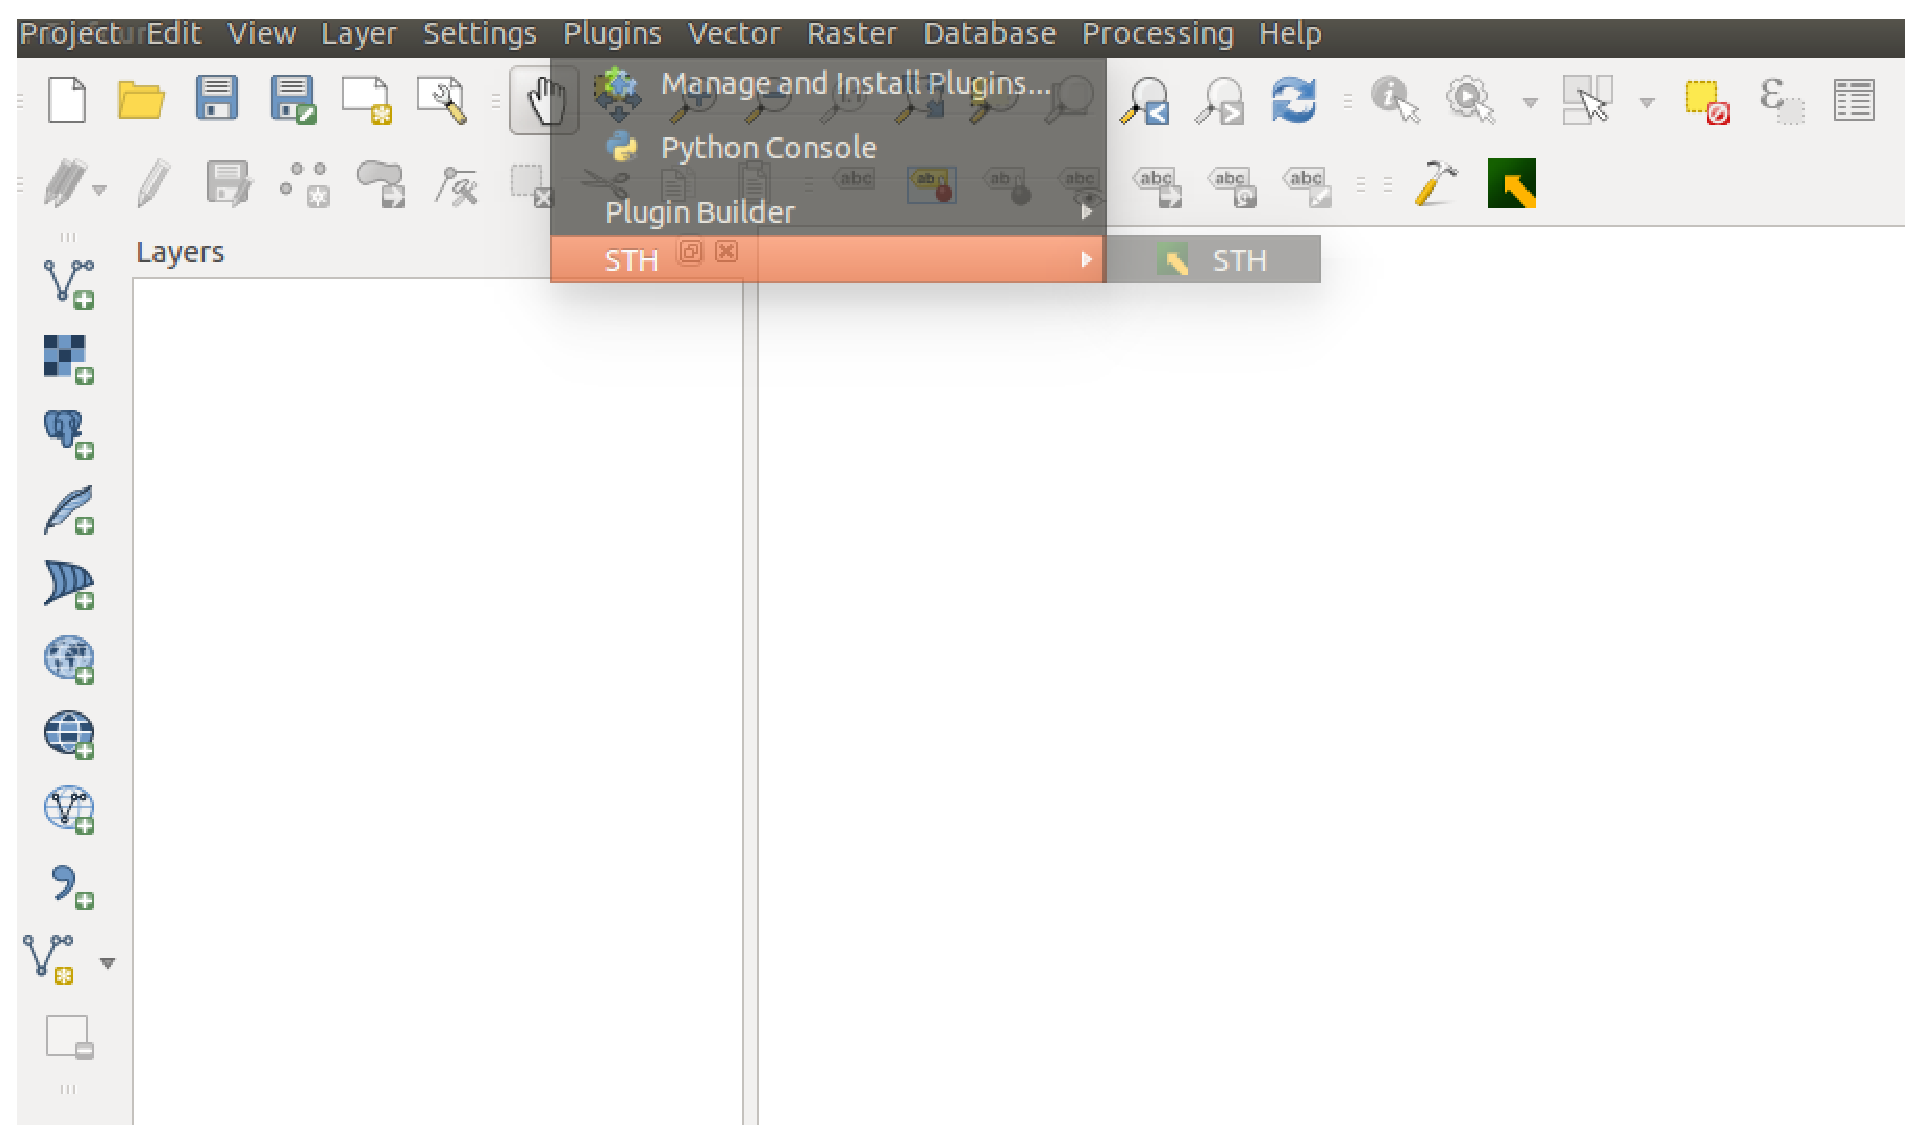
\includegraphics[scale=0.4]{sthscreen} 
\caption{Icon of STH-Predictor plugin} 
\label{sthscreen}
\end{figure}

\section*{2. Process and Application}
% \subsection{2.1. Process}
The main process can be seen in Figure \ref{mainprocess}. This figure shows the highest level of abstraction of the process, which encompasses three main sub-processes. The first sub-process is the task of users to prepare a proper input shapefile to be used with the STH-predictor. The second subprocess is about the plugin itself, which offers an users friendly interface to run the model. The third subprocess is with visualization and display of results obtained by running the model in previous step.

\begin{figure}[H]
\centering
\includegraphics[scale=0.4]{mainprocess} 
\caption{Main process} 
\label{mainprocess}
\end{figure}

\subsection{2.1. Prepare input shapefile}
This subprocess includes three main tasks (Figure \ref{input}):
\begin{figure}[H]
\centering
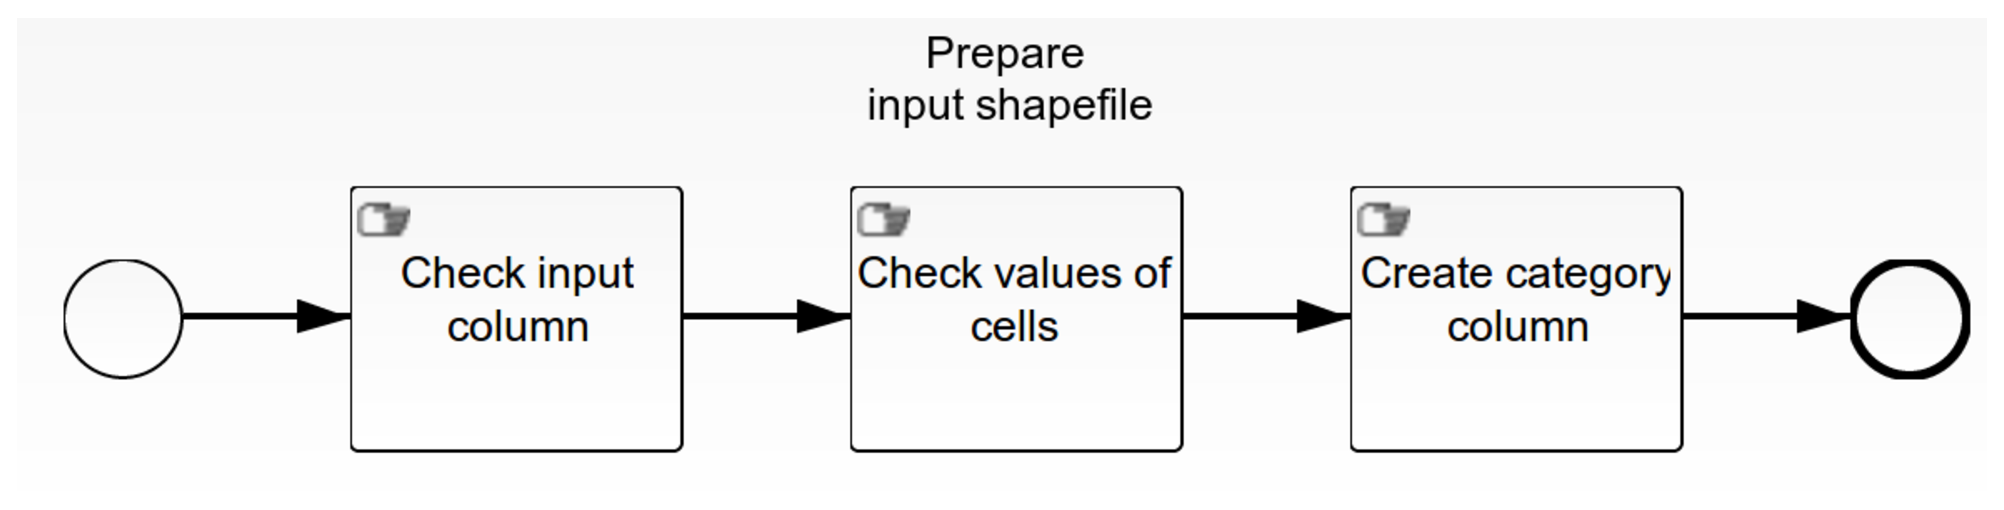
\includegraphics[scale=0.4]{input} 
\caption{Tasks to be prepared input shapefile} 
\label{input}
\end{figure}

\begin{itemize}
 \item \textbf{Check input column}: in a shapefile to be used with the STH-predictor plugin, there should exists 5 unique columns named ``CATEGORY'', ``STH'', ``HW'', ``Tt'', and ``Al''. If there is a missing of these columns, users are requested to create them. To create them, users can use QGIS to open the table of the shapefile and modify them. Other than using QGIS, users can use many commercial or open sources softwares to manipulate the attribute of shapefiles.
 \item \textbf{Check values of cells:} In each and every cells belong to each columns named ``CATEGORY'', ``STH'', ``HW'', ``Tt'', and ``Al'', there should be values. Under column ``CATEGORY'', cells must be filled in with categorical values ``A to F'' (e.g. A, B, C, D, E, F). This value is determined based on the value of column ``STH'' or the sum of three columns ``HW'', ``Tt'', and ``Al''. Values of cells in column ``STH'' are total prevalence recorded for each region shown in probability ranging from 0 to 1. Similarly, values of cells in columns ``HW'', ``Tt'', and ``Al'' are intensity values of ``Hookworms'', \textit{Trichuris trichiura}, and \textit{Ascaris lumbricoides}, respectively. 
 \item \textbf{Create category column:} If there ``CATEGORY'' is missing, users are required to create a column named ``CATEGORY'' for the selected shapefile. Then assign categorical values from ``A to F'' based on a rule that 1) category A is when total prevalence is less than 1\%; 2) category B is when total prevalence is in between [1,10\%);  3) category C is when total prevalence is in between [10,20\%); 4) category D is when total prevalence is in between [20,50\%); 5) category E is when total prevalance is in between [50,70\%); 6) category F is when total prevalence is greater than or equal to  70\%. 
\end{itemize}

In many practical situations, it is often that only total prevalence is available for each region. This means only values of cells of column ``STH'' are available. And values of cells in columns ``HW'', ``Tt'', and ``Al'' are partially or not available. The STH-predictor plugin still works perfectly. However, users are noted to not select the model for use with these situation. The default model to be run is when all cells of column ``STH'' receives values. 


A shapefile is a file with extension .shp. The .shp format is a widely used type of file supporting geospatial vector, which is used to display information on any GIS software \footnote{https://en.wikipedia.org/wiki/Shapefile}. In the context of prediction for STH, the shapefile is defined with polygon structure. Each polygon represents an administrative management region, in which, the information related to prevalence of the STH is recorded. 

For example, in Figure \ref{indianmap}, each polygon represents a provincial region of India. 

\begin{figure}[H]
\centering
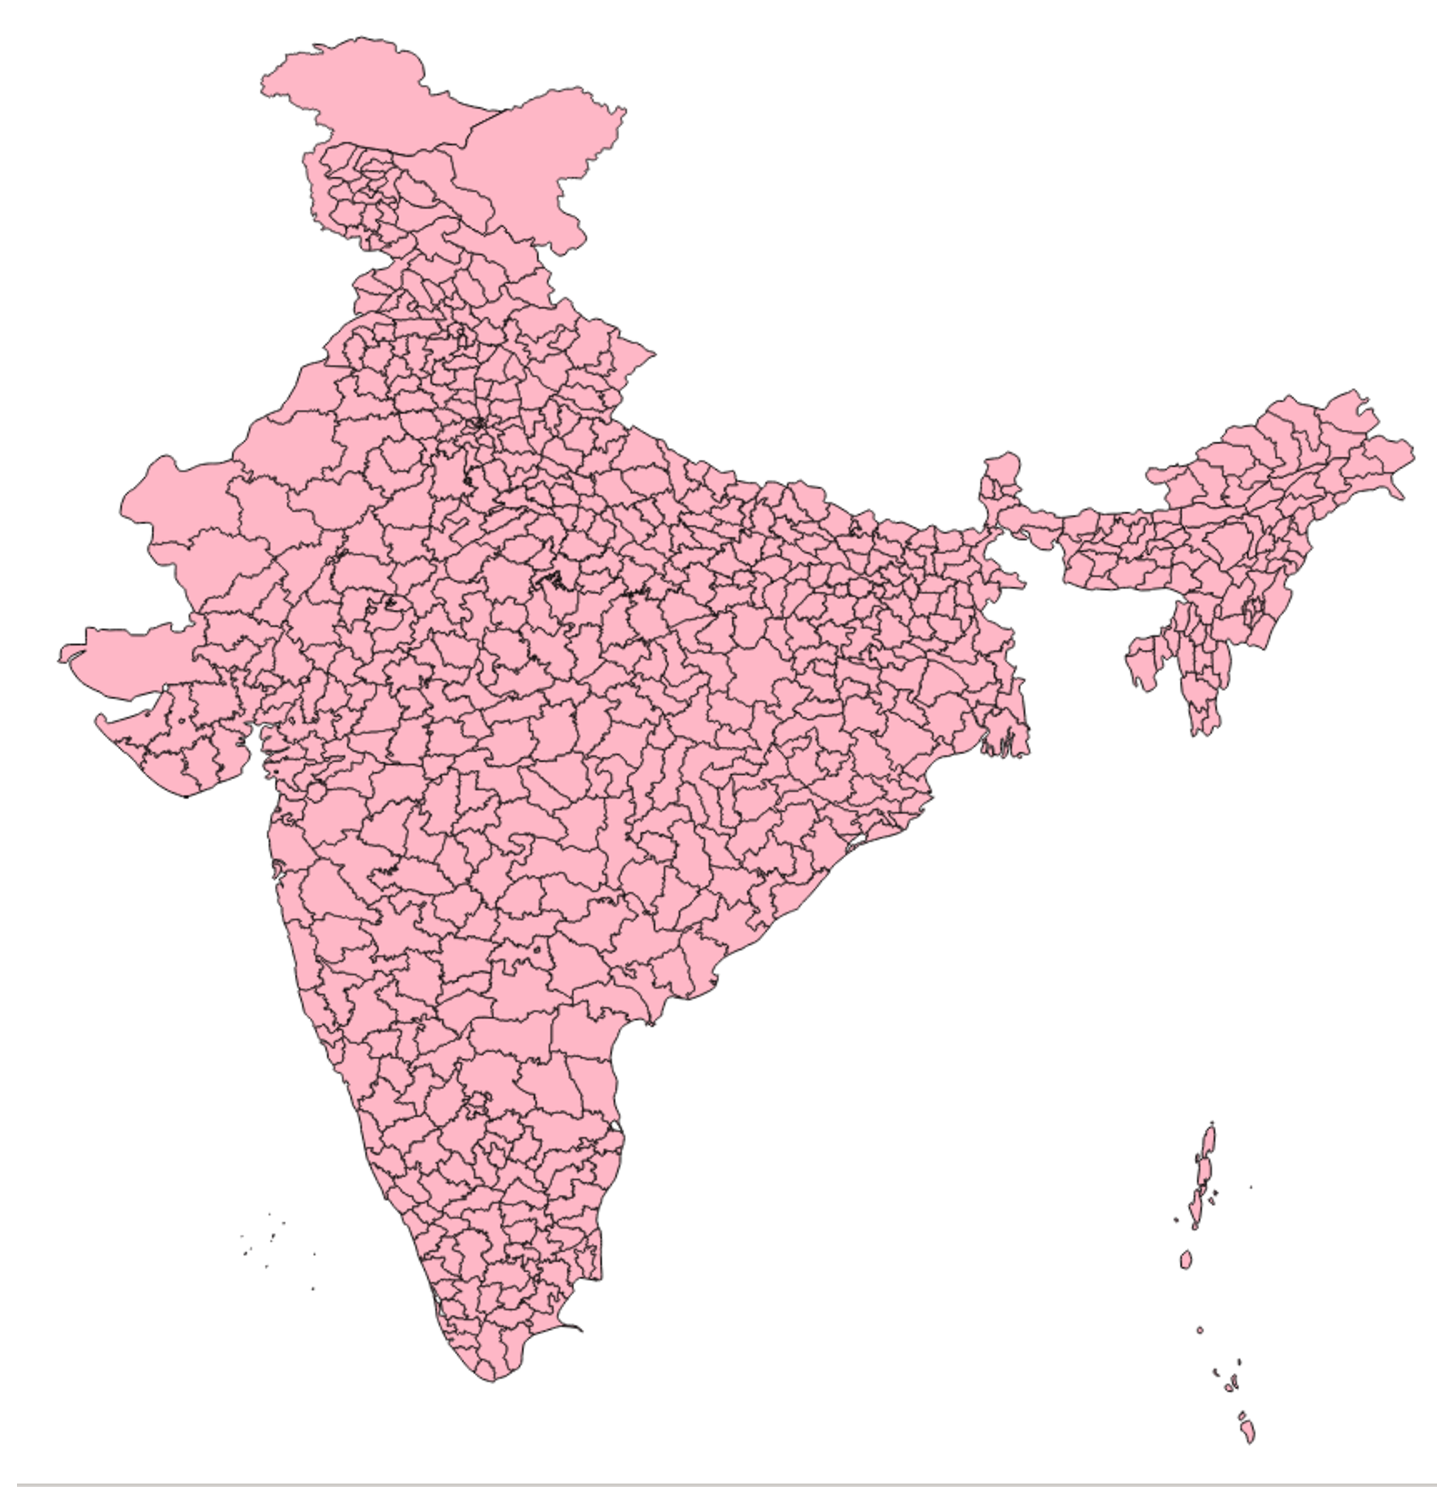
\includegraphics[scale=0.3]{indianmap} 
\caption{Map of provincial regions of India in Polygon structure} 
\label{indianmap}
\end{figure}

In order for the shapefile to be workable, a shapefile itself is linked to additional 3 files, which always come together with the shapefile and they are being created automatically whenever a shapefile is created. Therefore, it is important to note that whenever users want to copy/more a shapefile, they must copy/more all 4 files together and place them exactly in a same working folder. For example, the folder containing input.shp file shown in Figure \ref{inputshapefile} contains also three additional files with extensions .prj, .dbf, and .shx, respectively. 

\begin{figure}[H]
\centering
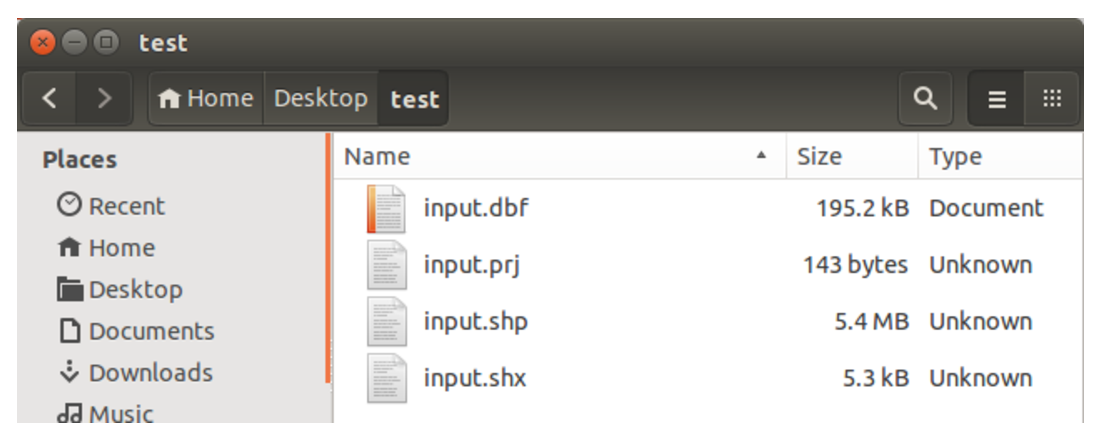
\includegraphics[scale=0.5]{inputshapefile} 
\caption{Folder contains shapefile and its associate files} 
\label{inputshapefile}
\end{figure}

Using QGIS, users can add the shapefile into its working environment and display the properties of the selected shapefile. Figure \ref{shapfileattribute} shows the structure of a shapefile containing the information of total prevalence of STH and intensities of each STH's species.

\begin{figure}[H]
\centering
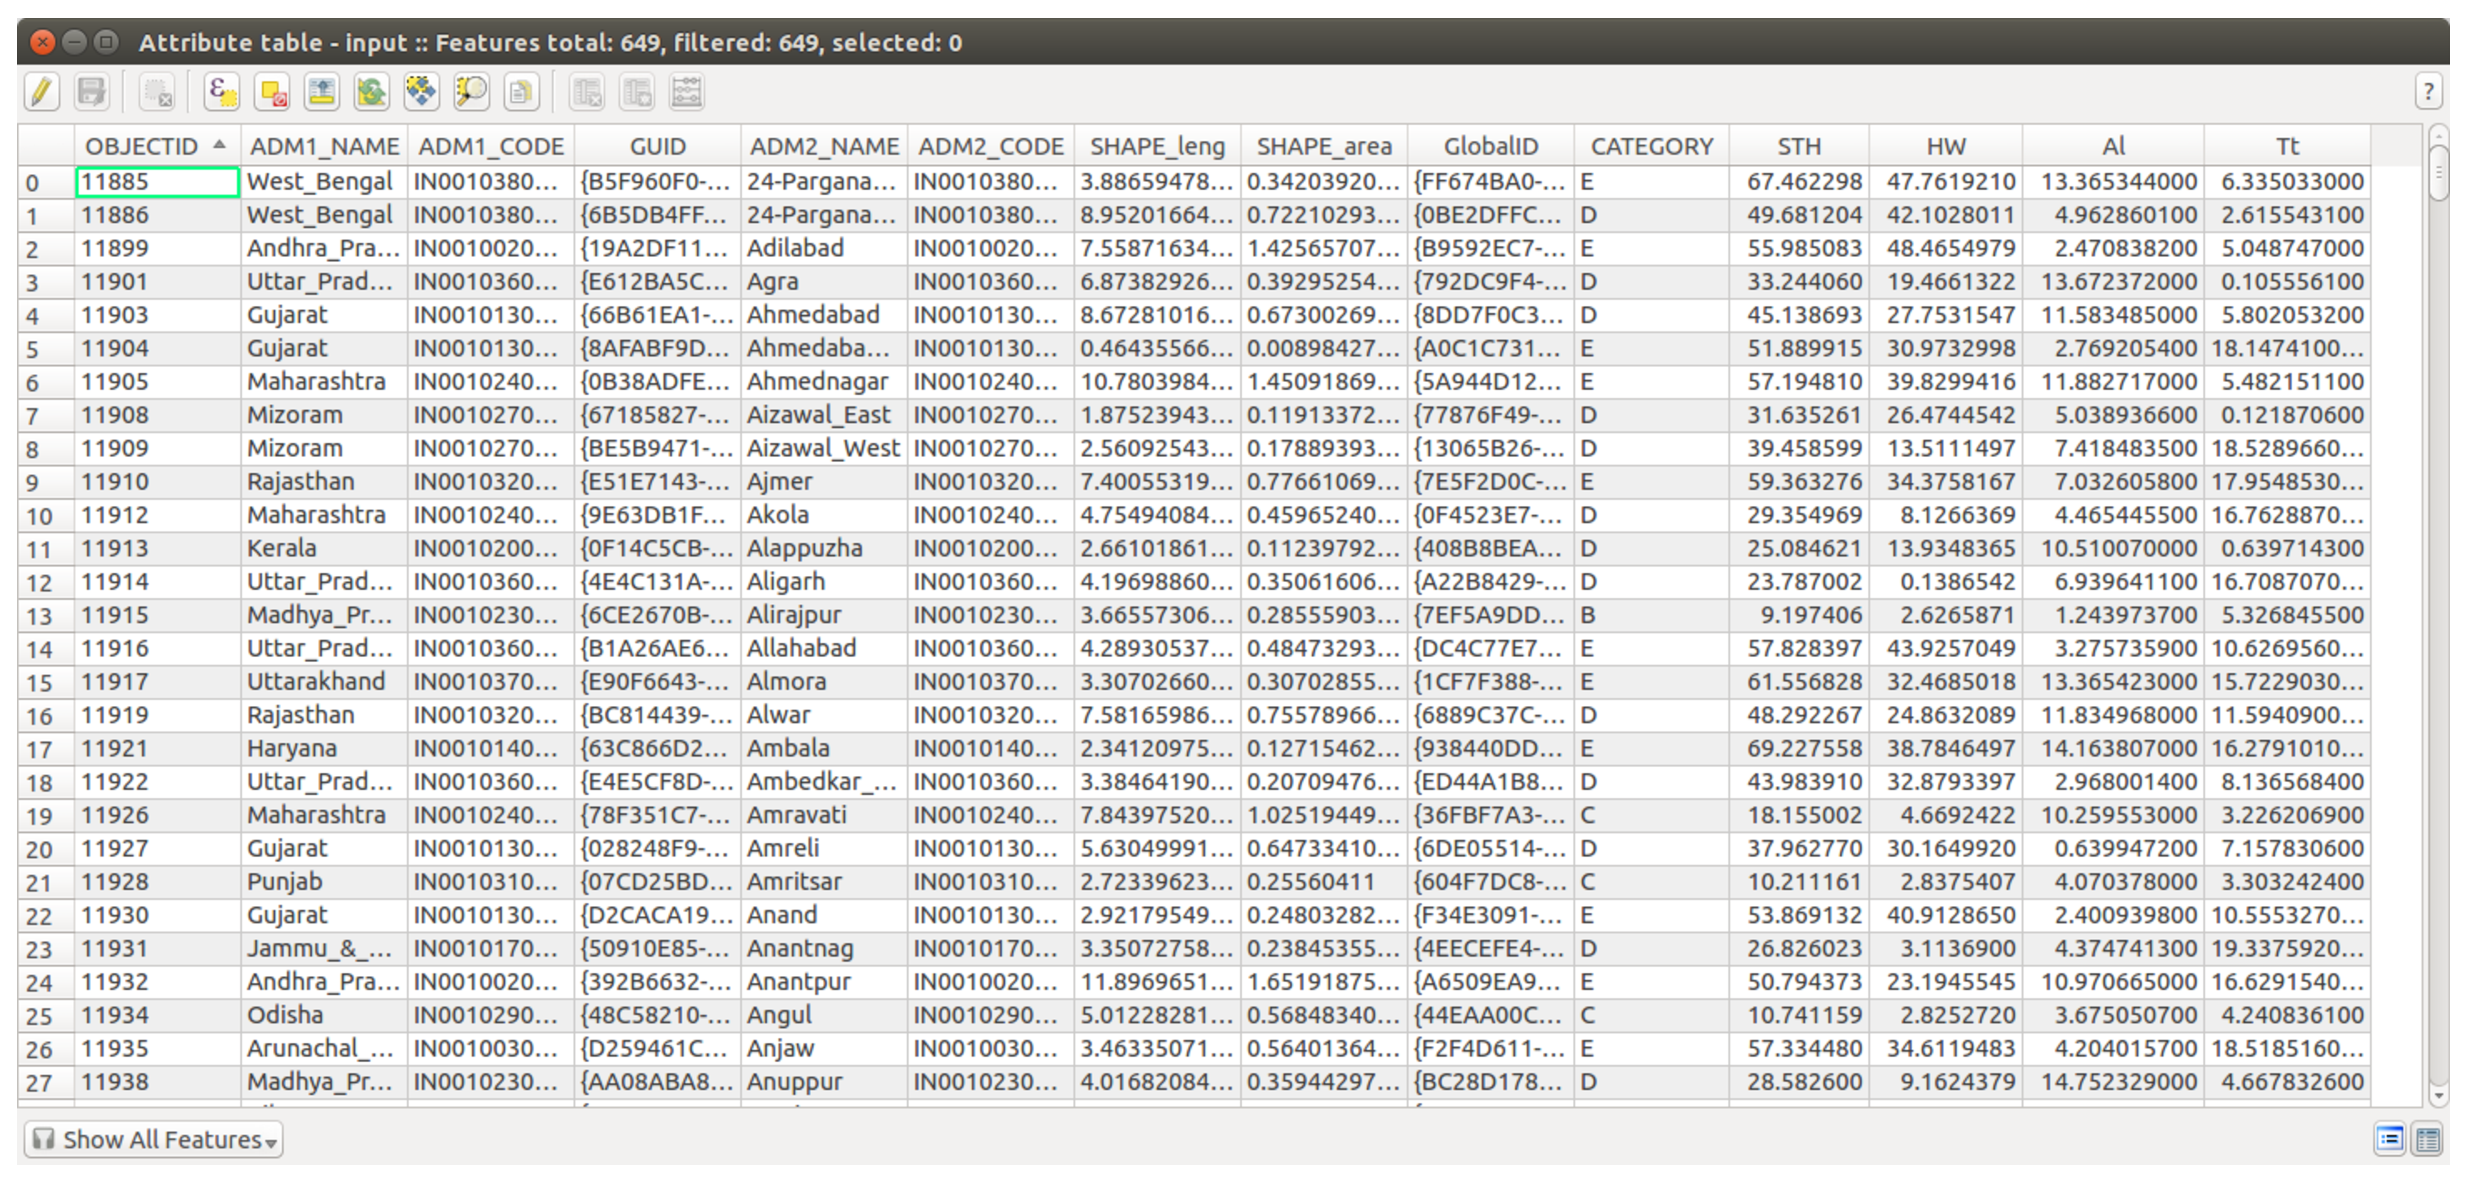
\includegraphics[scale=0.4]{shapfileattribute} 
\caption{Attributes of a shapefile used for prediction with the STH-predictor} 
\label{shapfileattribute}
\end{figure}

As can be seen in the figure, the first 9 columns of the tables is always come with the shapefile itself and the users should not delete or change it. Information of these columns is nowadays defined as a standard. This information is issued by the government of India. In any other country, this information is more or less similar and can be down loadable via various Internet portals.

The last 5 columns is important for users of the STH-predictor. Values of cells under each column must be created/recorded by users. In practical situation, many local district or provincial personnel record data using spreadsheet such as MS Excel application. Such recorded data can be imported directly into shapefile. 

If the user's shapefile does not contain such 5 columns, users must create them by using QGIS. Steps to create them are as followed

\begin{itemize}
 \item \textbf{Step 1: Load input shapefile:} Click icon \Addvector{} (add vector layer) on the left panel of the QGIS (or go to \textbf{Layer --$>$ Add Vector Layer}). (Figre \ref{addvector})
 \begin{figure}[H]
\centering
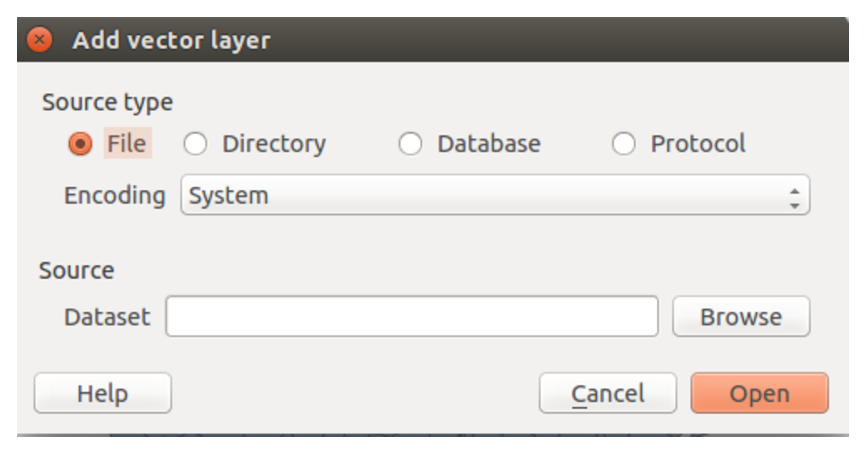
\includegraphics[scale=0.5]{addvector} 
\caption{Add vector layer (QGIS)} 
\label{addvector}
\end{figure}
 Click button ``\textbf{Browse}'' and navigate to folder containing the input shapefile, then select the input shapefile ending with .shp format.
 
 One the shapefile is opened, a map will appear in random color. Following figure (Figure \ref{indianmaprandom}) shows the map of India, with all its regions. Each region is represented by a polygon. 

\begin{figure}[H]
\centering
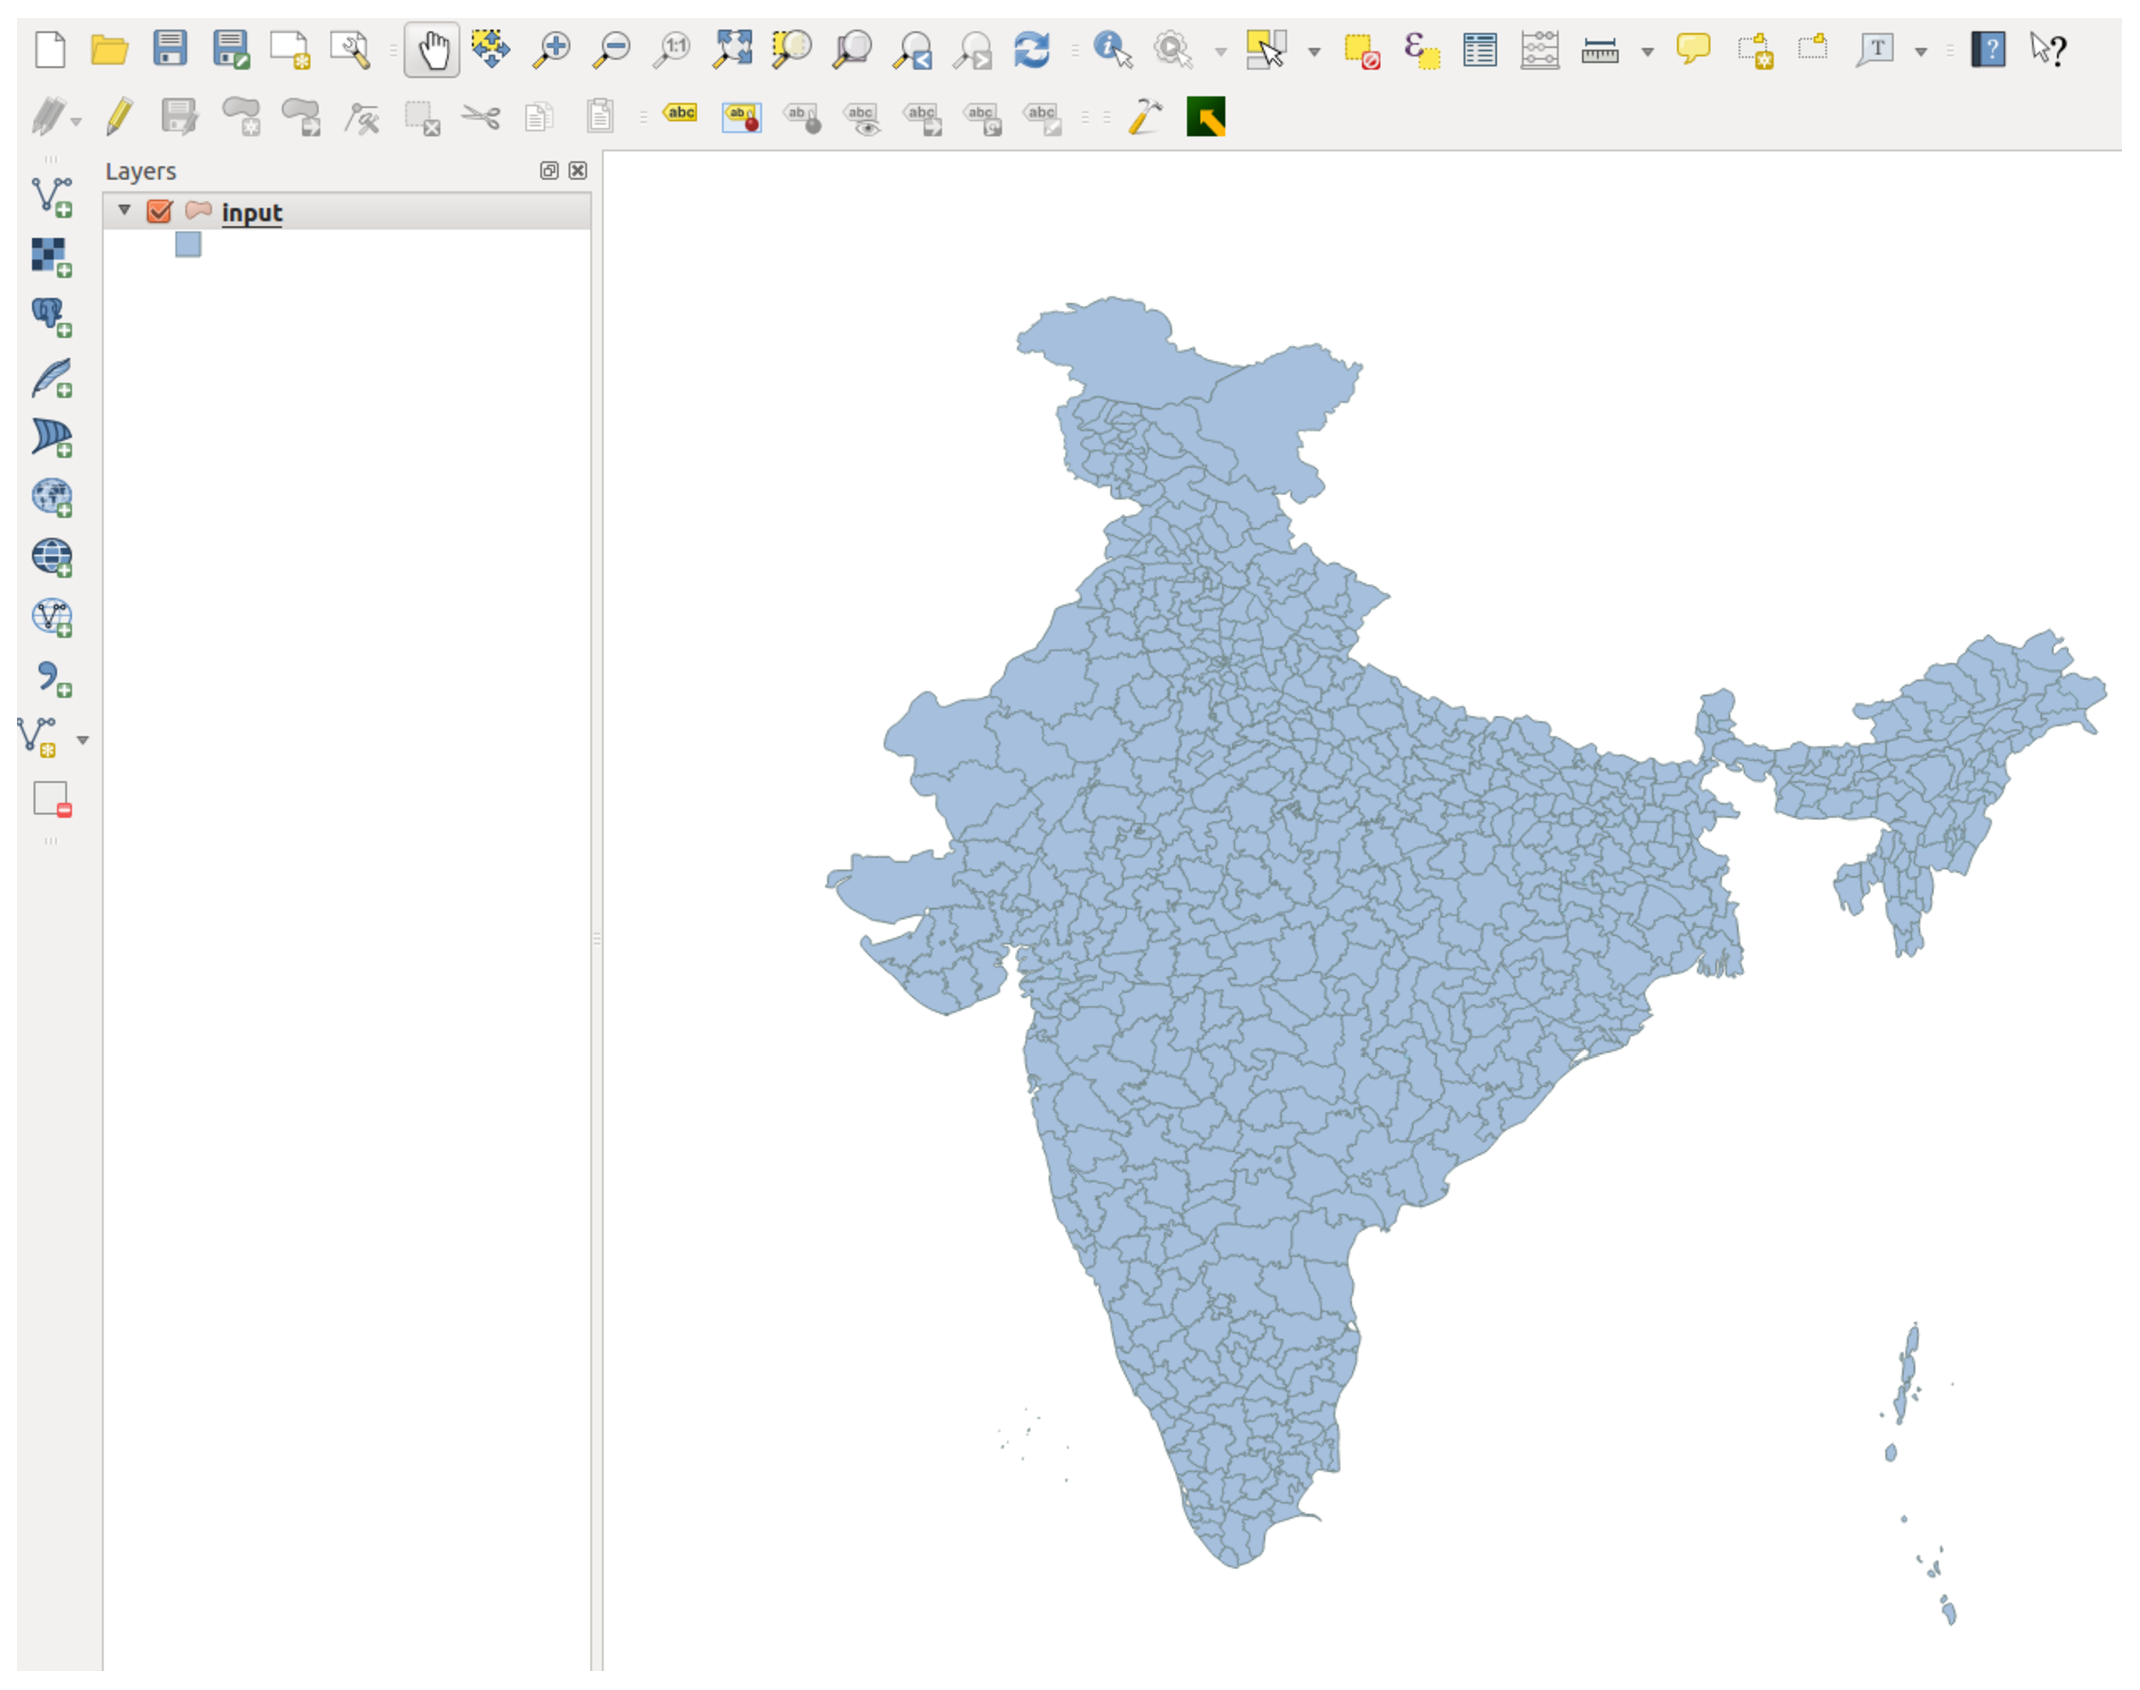
\includegraphics[scale=0.3]{indianmaprandom} 
\caption{Map of india with all its regions} 
\label{indianmaprandom}
\end{figure}

 \item \textbf{Step 2: Open attribute table:} Click icon \openatt{} (Open Attribute Table) on QGIS main panel (or go to \textbf{Layer --$>$ Open Attribute Table}). 
 
 The table of the shapefile will be appeared and look like the one shown in Figure \ref{shapfileattribute}. If any column with name ``CATEGORY'', ``STH'', ``HW'', ``Tt'', or ``Al'' is missing, users can create them within QGIS table attribute environment.
 
 + In Figure \ref{shapfileattribute}, Click icon pencil \openpen{} located on the top left corner of attribute table. All icons of the attribute table (Figure \ref{tablemenu}) will be visible and users can click on each of them for editing the data.
 
 \begin{figure}[H]
\centering

\includegraphics[scale=0.7]{tablemenu} 
\caption{Icons of attribute table} 
\label{tablemenu}
\end{figure}
 
The last three icons shown in Figure \ref{tablemenu} are used to delete, create, and manipulate columns of the table. Users of the STH-predictor are advised to read some basic concepts and steps in order to manipulate vector data shapefiles from QGIS documentation repository such as the user guide manual (QGIS2.2) \footnote{https://docs.qgis.org/2.2/en/docs/user\_manual/index.html}
 
Following code is given for users to assign categorical values to column ``CATEGORY'' when using the last icon of Figure \ref{tablemenu} to manipulate the data of the table (Figure \ref{manipulatetable}).

\begin{lstlisting}[basicstyle=\tiny,style=nonumbers]
CASE 
	WHEN STH < 1 THEN 'A' 
	WHEN STH < 10 THEN 'B' 
	WHEN STH < 20 THEN 'C' 
	WHEN STH < 50 THEN 'D' 
	WHEN STH < 70 THEN 'E' 
	ELSE 'F'
END
\end{lstlisting}

\begin{figure}[H]
\centering
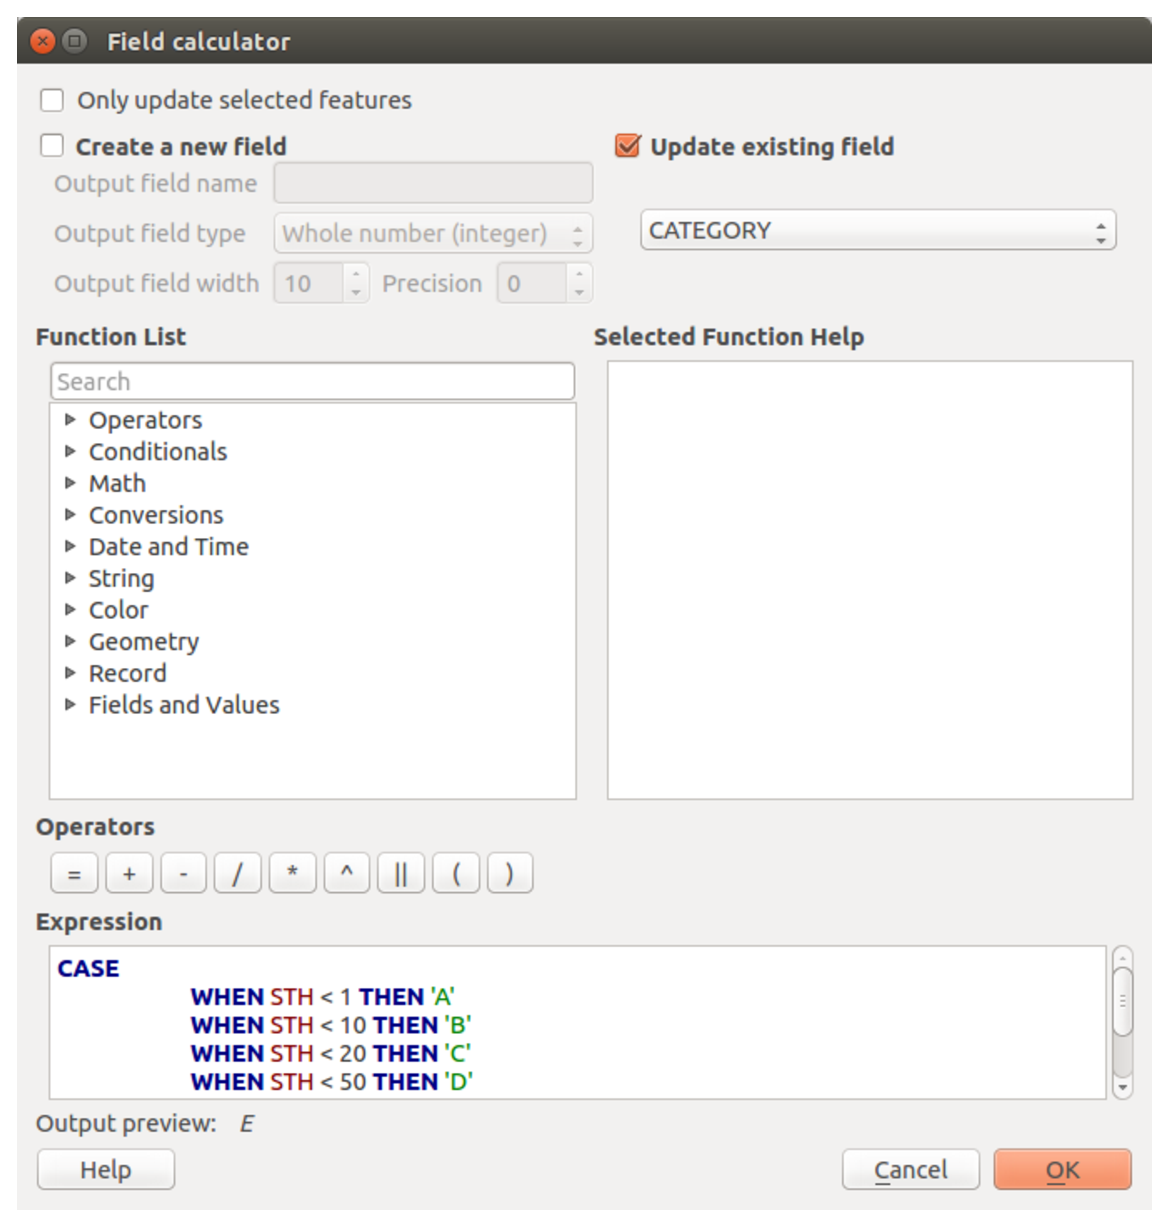
\includegraphics[scale=0.35]{manipulatetable} 
\caption{Field calculator for the attribute table} 
\label{manipulatetable}
\end{figure}

\item \textbf{Step 3: Display prevalence on the map:} By open the ``Properties'' of Input layer and Load the color style (as shown in Figure \ref{propertyboxgraduate}). A map of prevalance of input will appear as shown in Figure \ref{indianmapinput}.
\begin{figure}[H]
\centering
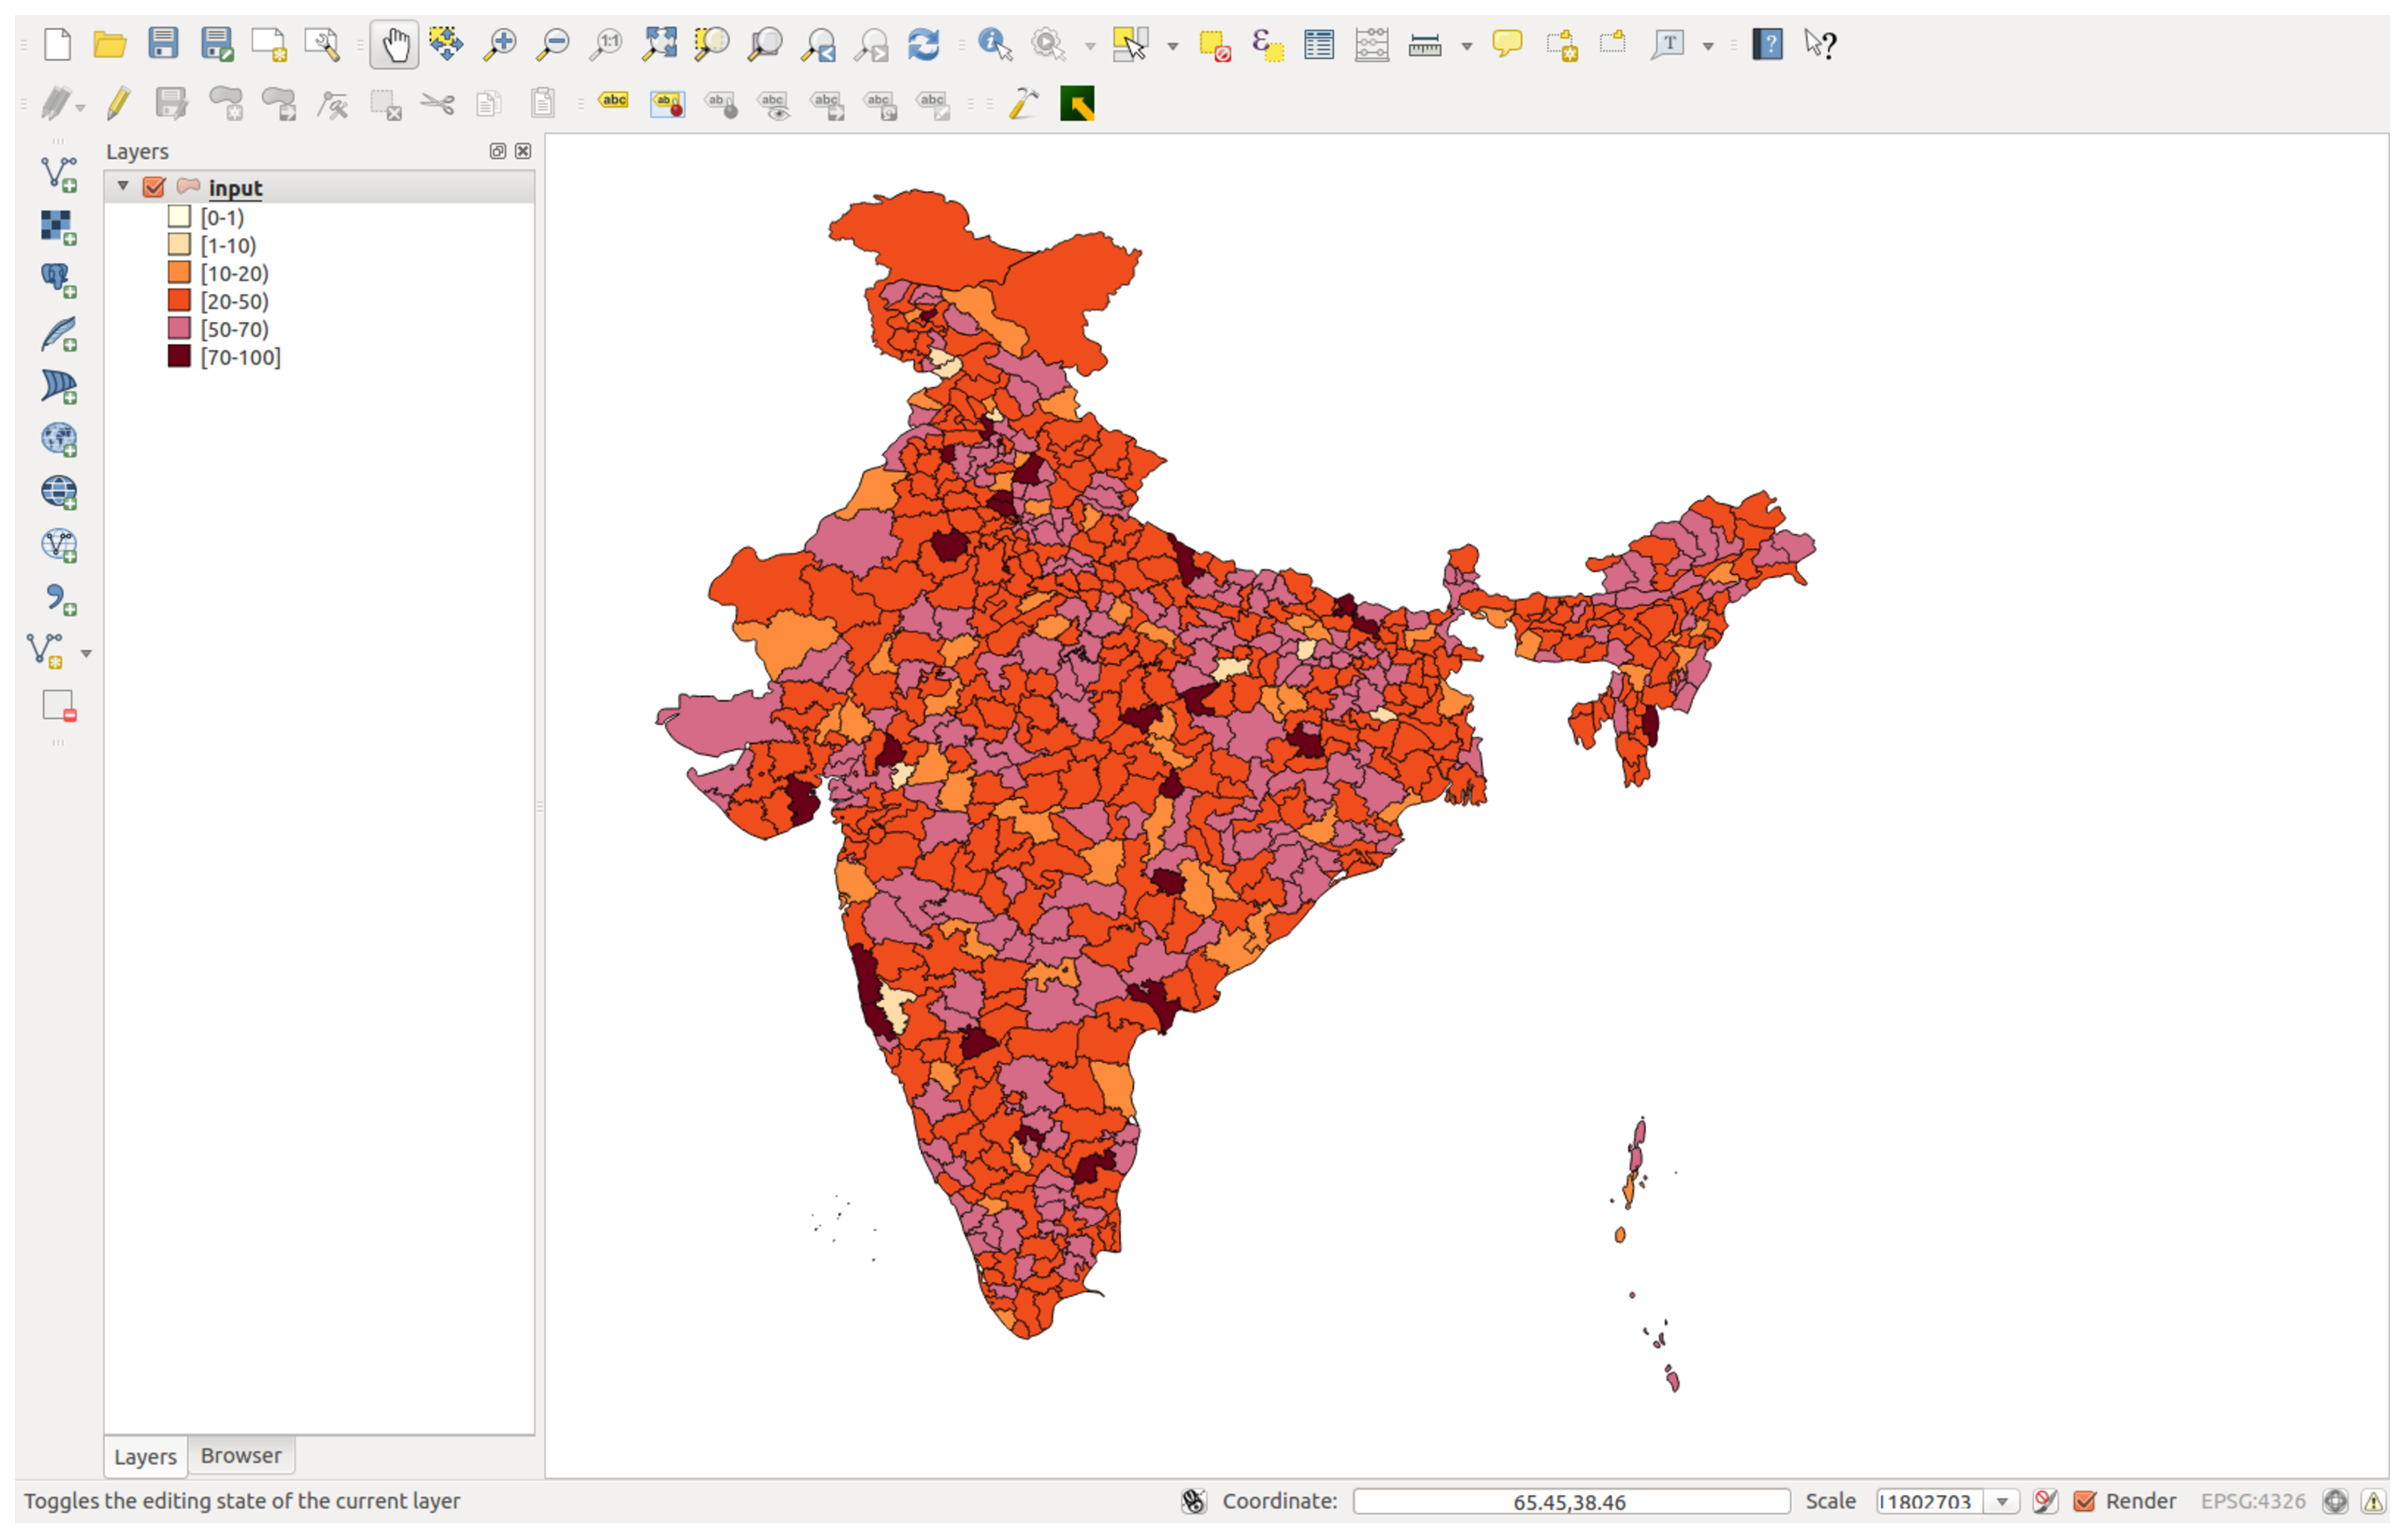
\includegraphics[scale=0.3]{indianmapinput} 
\caption{Prevalence map of India} 
\label{indianmapinput}
\end{figure}


The default color style for the STH-predictor is saved in sub-folder named ``colorstyles'' of the main plugin STH-predictor folder
\begin{figure}[H]
\centering
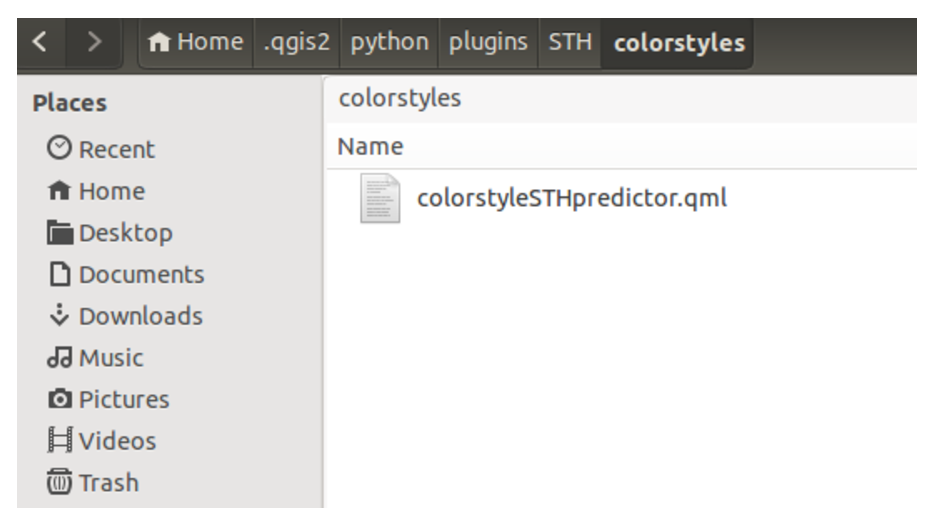
\includegraphics[scale=0.5]{colorstylefolder} 
\caption{Color style file saved in STH-predictor plugin folder} 
\label{colorstylefolder}
\end{figure}

\end{itemize}


\subsection{2.2. Run the model}
To run the model on a specific shapefile, users are required to perform sequential or parallel tasks shown in the diagram of Figure \ref{runmodel}. 
\begin{figure}[H]
\centering
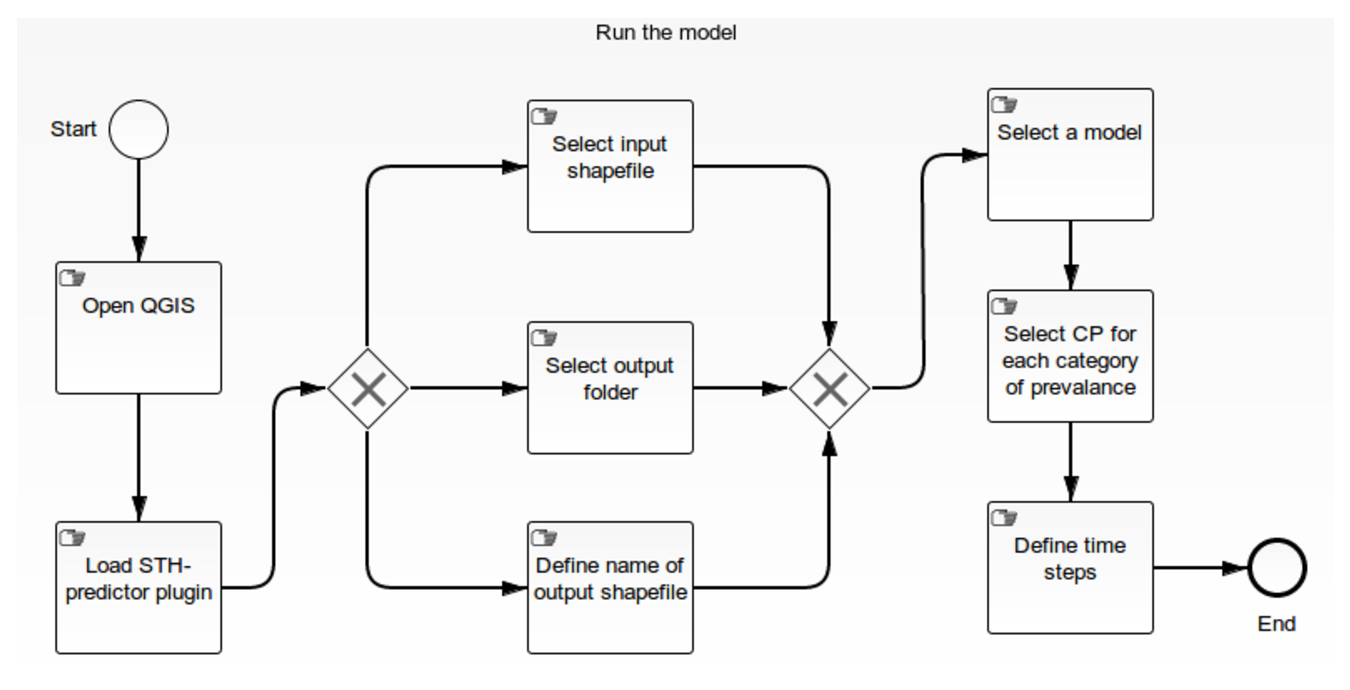
\includegraphics[scale=0.6]{runmodel} 
\caption{Run the model} 
\label{runmodel}
\end{figure}

\subsubsection{Open QGIS}
If a version of QGIS has been installed in your operation system, users can find the softwares easily in the program panel.
\subsubsection{Load STH-predictor plugin}
By clicking the icon of the STH-predictor, the STH-predictor will be loaded automatically and its interface will appear on the screen (Figure \ref{sthwelcome}).
\begin{figure}[H]
\centering
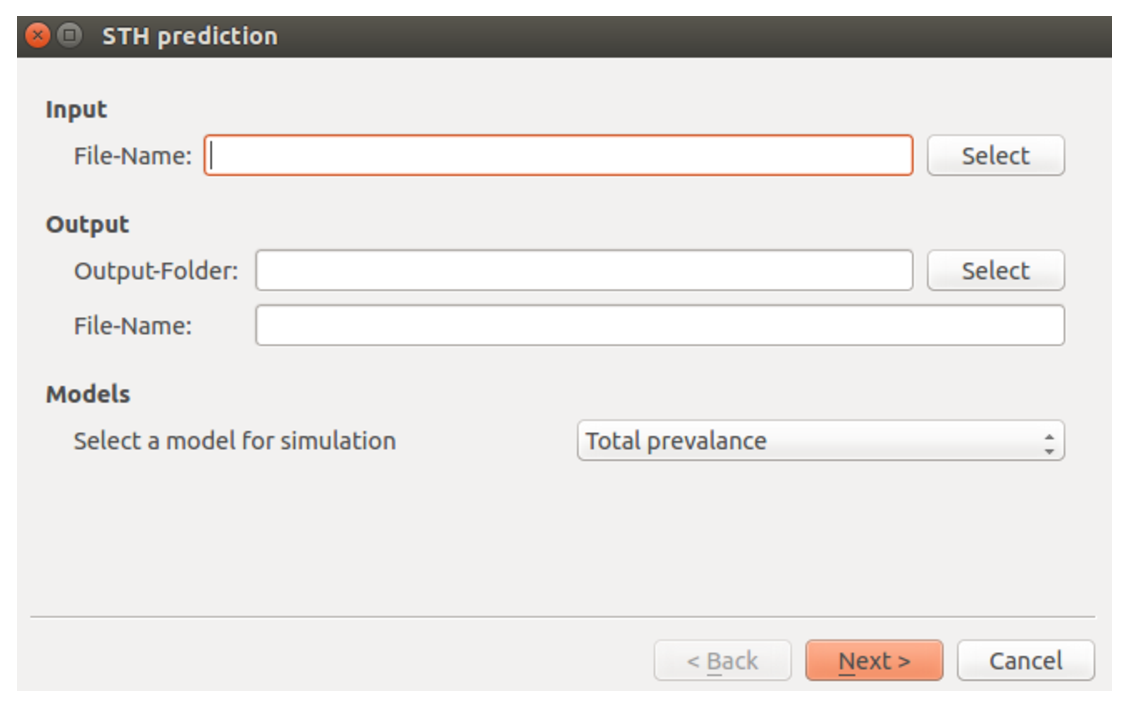
\includegraphics[scale=0.5]{sthwelcome} 
\caption{Welcome screen} 
\label{sthwelcome}
\end{figure}

\subsubsection{Select input shapefile}
By clicking the ``select'' button in the input section, users can navigate to the folder containing the shapefile file and choose it (Figure \ref{sthselection}).

\begin{figure}[H]
\centering
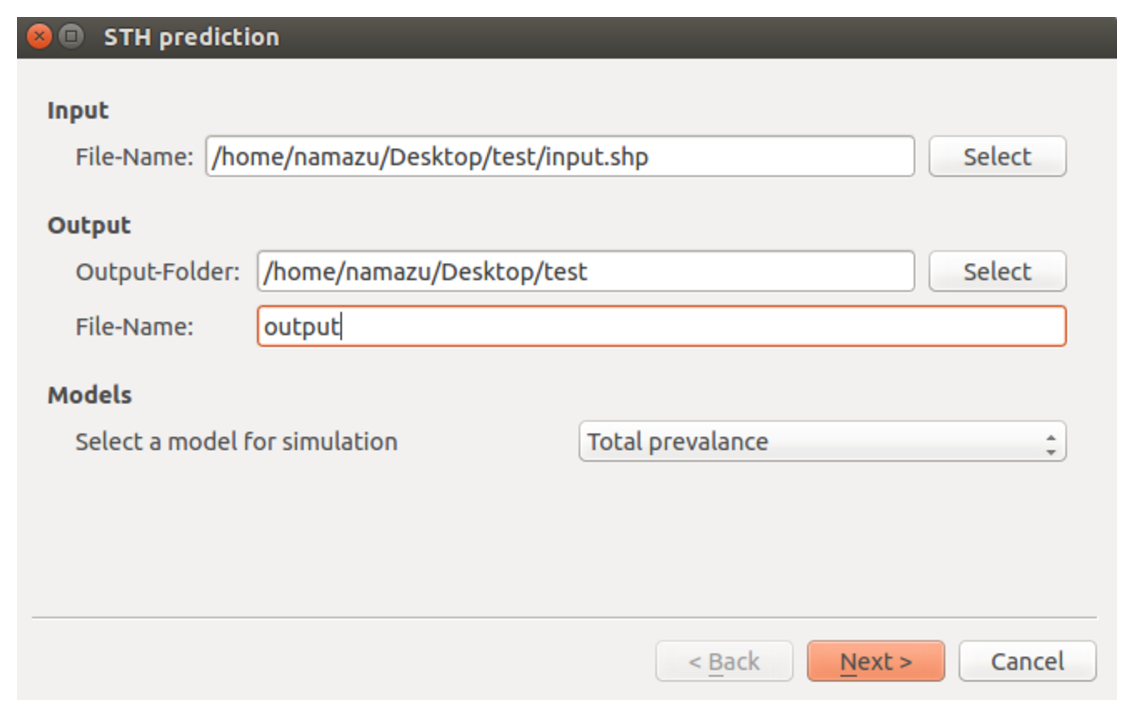
\includegraphics[scale=0.5]{sthselection} 
\caption{Input and output selection} 
\label{sthselection}
\end{figure}

\subsubsection{Select output folder}
By clicking the ``select'' button in the output section, users can navigate to the folder, in which, users would like to save the output shapefiles (Figure \ref{sthselection}).

\subsubsection{Define name of output shapefile}
name of output's shapefile can be typed inside the box ``file-name''. Users do not need to specify the extension format of the shapefile (e.g. output.shp), the program itself will create automatically shapefiles and stored them in the selected output folder (Figure \ref{sthselection}). 
\subsubsection{Select a model}
In this step, users need to decide which models they want to use for prediction. There are two models built in the plug-in. The default model is used when there is only information of total prevalence of the STH. The other model is when information of intensity of  Hookworms, \textit{Trichuris trichiura}, and \textit{Ascaris lumbricoides} is available. 

Once a model is selected, users can move forward by clicking ``Next'' button shown in the Figure \ref{sthselection}.
\subsubsection{Select control program (CP) for each category}
When the ``Next'' button shown in the Figure \ref{sthselection} is selected, a new interface will appear. This interface gives users choices to select which control program (CP) to be used under 6 categories mentioned earlier. 

\begin{figure}[H]
\centering
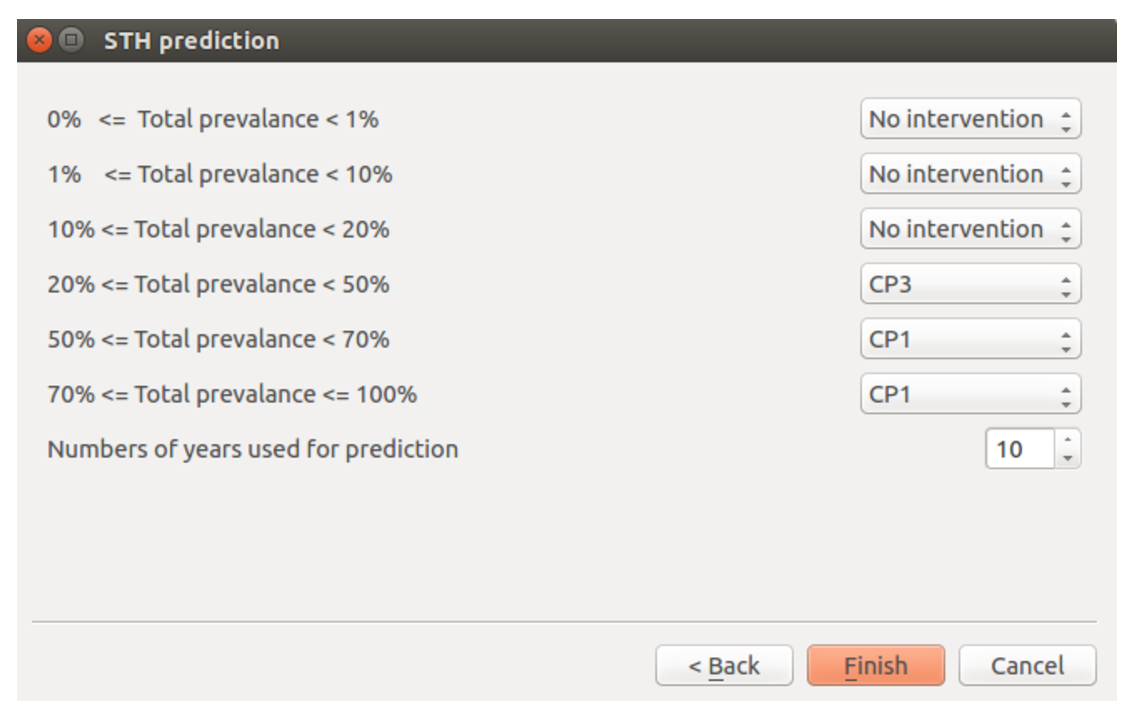
\includegraphics[scale=0.5]{cpselection} 
\caption{Select the control program} 
\label{cpselection}
\end{figure}

The default CP for each category is automatically appeared. This default CP is set based on expert opinion. However, users can define a CP differently from the default one. 

To choose another CP other than the default one, users can click and choose CPs from com-box box under each category.

When users move cursor over each com-box box, a tool-tip text will appear and give users the definition of each CP. 

The definition of each CP is given below.

\begin{itemize}
 \item \textbf{No intervention:} when no drug is distributed. Under this situation, the distribution of prevalence in future will not change. 
 \item \textbf{CP1 (Administration of anthelminthic (ALB)  twice a year):} The STH control program is consisting on the administration twice a year of a tablet of albendazole (400 mg) to all school-age children. The drug administration is normally organized using the school infrastructure, also the children of school age that are not enrolled in school are offered drug. School children absent the day of the drug administration are provided the drug when they return to school.
 \item \textbf{CP2 ( Administration of anthelminthic (MEB)  twice a year):} The STH control program is consisting on the administration twice a year of a tablet  of mebendazole (500 mg) to all school-age children. The drug administration is normally organized using the school infrastructure, also the children of school age that are not enrolled in school are offered drug. School children absent the day of the drug administration are provided the drug when they return to school.
 \item \textbf{CP3 (Administration of anthelminthic (ALB) once a year):} The STH control program is consisting on the administration once a year of a tablets of albendazole (400 mg ) to all school-age children. The drug administration is normally organized using the school infrastructure, also the children of school age that are not enrolled in school are offered drug. School children absent the day of the drug administration are provided the drug when they return to school. 
 \item \textbf{CP4 (Administration of anthelminthic (MEB) once a year):} The STH control programme is consisting on the administration once a year of a tablets of mebendazole (500 mg ) to all school-age children. The drug administration is normally organized using the school infrastructure, also the children of school age that are not enrolled in school are offered drug. School children absent the day of the drug administration are provided the drug when they return to school.
 \item \textbf{CP5 (Administration of anthelminthic for STH in the context of lymphatic filariasis (LF) control program:  administration of drug for LF (albendazole + ivermectin) + ALB  at six months interval from the LF intervention):} The STH control programme is integrated with the control of Lymphatic Filariasis. The drug administration is based on the administration once a year of albendazole (400 mg) and ivermectin (150 $\mu$g/Kg) to the entire population plus the administration, at approximately 6 months of interval, of albendazole (400mg) to all school age children.
 \item \textbf{CP6 (Administration of anthelminthic for STH in the context of lymphatic filariasis (LF) control program: administration of drug for LF (albendazole + ivermectin) + MEB  at six months interval from the LF intervention):} The STH control programme is integrated with the control of Lymphatic Filariasis. The drug administration is based on the administration once a year of albendazole (400 mg) and ivermectin (150 $\mu$g/Kg) to the entire population plus the administration, at approximately 6 months of interval, of mebendazole (500mg) to all school age children.
 \item \textbf{CP7 (Administration of anthelminthic for STH in the context of lymphatic filariasis (LF) control program: (ALB)  at six months interval from the administration of drug for LF (albendazole + DEC) ):} The STH control program is integrated with the control of Lymphatic Filariasis. The intervention is based on the administration once a year of albendazole (400 mg) and dyethilcarbamazine (6 mg/Kg) to the entire population plus the administration of albendazole (500mg) to all school age children.
 \item \textbf{CP8 (Administration of anthelminthic for STH in the context of lymphatic filariasis (LF) control program: (MEB)  at six months interval from the administration of drug for LF (albendazole + DEC) ):} The STH control program is integrated with the control of Lymphatic Filariasis. The intervention is based on the administration once a year of albendazole (400 mg) and dyethilcarbamazine (6 mg/Kg) to the entire population plus the administration of albendazole (500mg) to all school age children.
 \item \textbf{CP9 (Administration of anthelminthic for STH in the context of lymphatic filariasis (LF) control program: administration of drug for LF (albendazole + DEC)  only ):} The STH control program is already covered by the control of Lymphatic Filariasis. The intervention is based on the administration once a year of albendazole (400 mg) and dyethilcarbamazine (6 mg/Kg).
 \item \textbf{CP10 (Administration of anthelminthic for STH in the context of lymphatic filariasis (LF) control program: administration of drug for LF (albendazole + IVR)  only ):} The STH control program is already covered by the control of Lymphatic Filariasis. The intervention is based on the administration once a year of albendazole (400 mg) and ivermectin (150 $\mu$g/Kg).
\end{itemize}

\subsubsection{Define time steps}
This is the last step with the modeling section. Users can choose the time intervals (in years) for prediction. The default time intervals is 10 years (Figure \ref{cpselection}) as it is convinced that a period of 10 years is good enough for prediction and decision making regarding the determination of the optimal set of control programs. 

After selecting the time interval, users can click the button ``Finish'' shown in Figure \ref{cpselection} to complete the task.
\subsection{2.3. Display results}
Once users click the button ``Finish'' shown in Figure \ref{cpselection}, the program will perform calculation and prediction. Results of this process will be automatically recorded in the output shapefile, which users have chosen earlier. 

Both input and output shapefiles are loaded in QGIS environment and attributes of fields in each shapefile can be displayed as maps, with different color for the purposes of visualization and reporting. 

The steps in displaying results are depicted in Figure \ref{output}.

\begin{figure}[H]
\centering
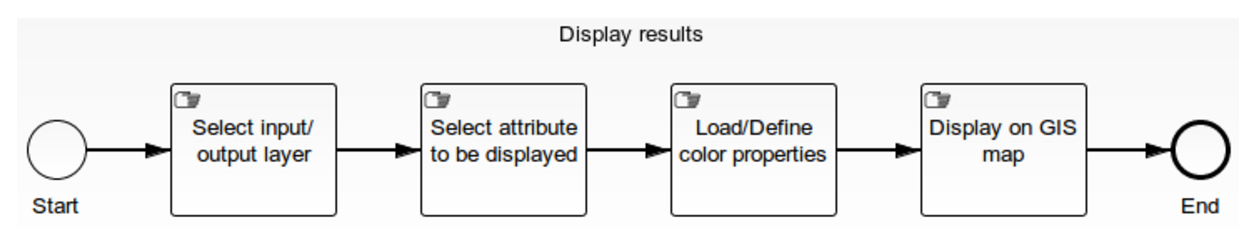
\includegraphics[scale=0.8]{output} 
\caption{Display results} 
\label{output}
\end{figure}
\subsubsection{Select input/output layer}
Under layer panel of QGIS, users can choose the layer, which is basically the input or output shapefile, to be shown as map in the main window. 
\subsubsection{Select attribute to be displayed}
Move the cursor to the layer (e.g. input) and select it, \textbf{Right Click} on the selected layer and then select ``Properties'' (As shown in Figure \ref{outputattributeselect})
\begin{figure}[H]
\centering
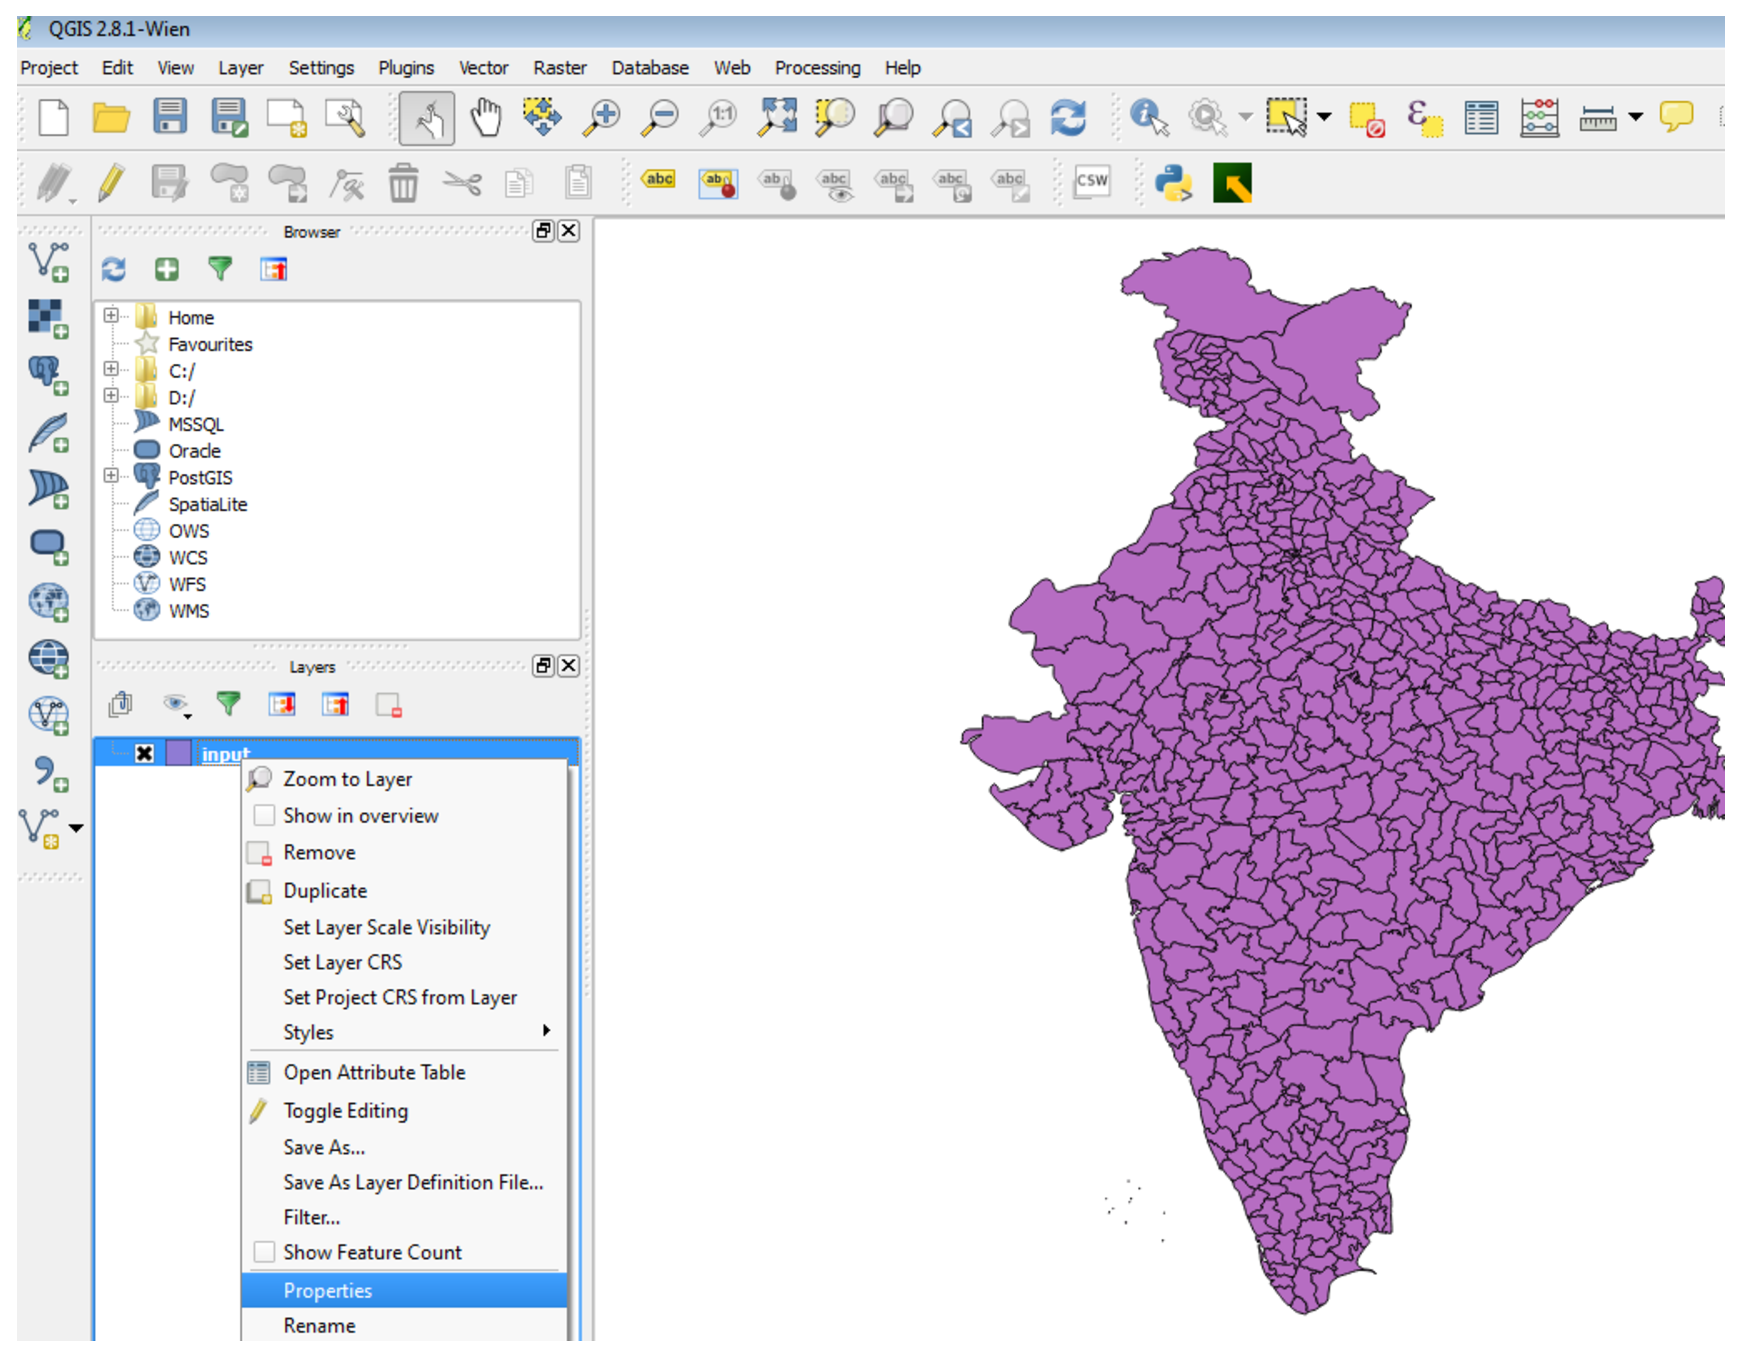
\includegraphics[scale=0.4]{outputattributeselect} 
\caption{Select properties of layer} 
\label{outputattributeselect}
\end{figure}

The properties box will appears as shown in Figure \ref{propertybox}.

\begin{figure}[H]
\centering
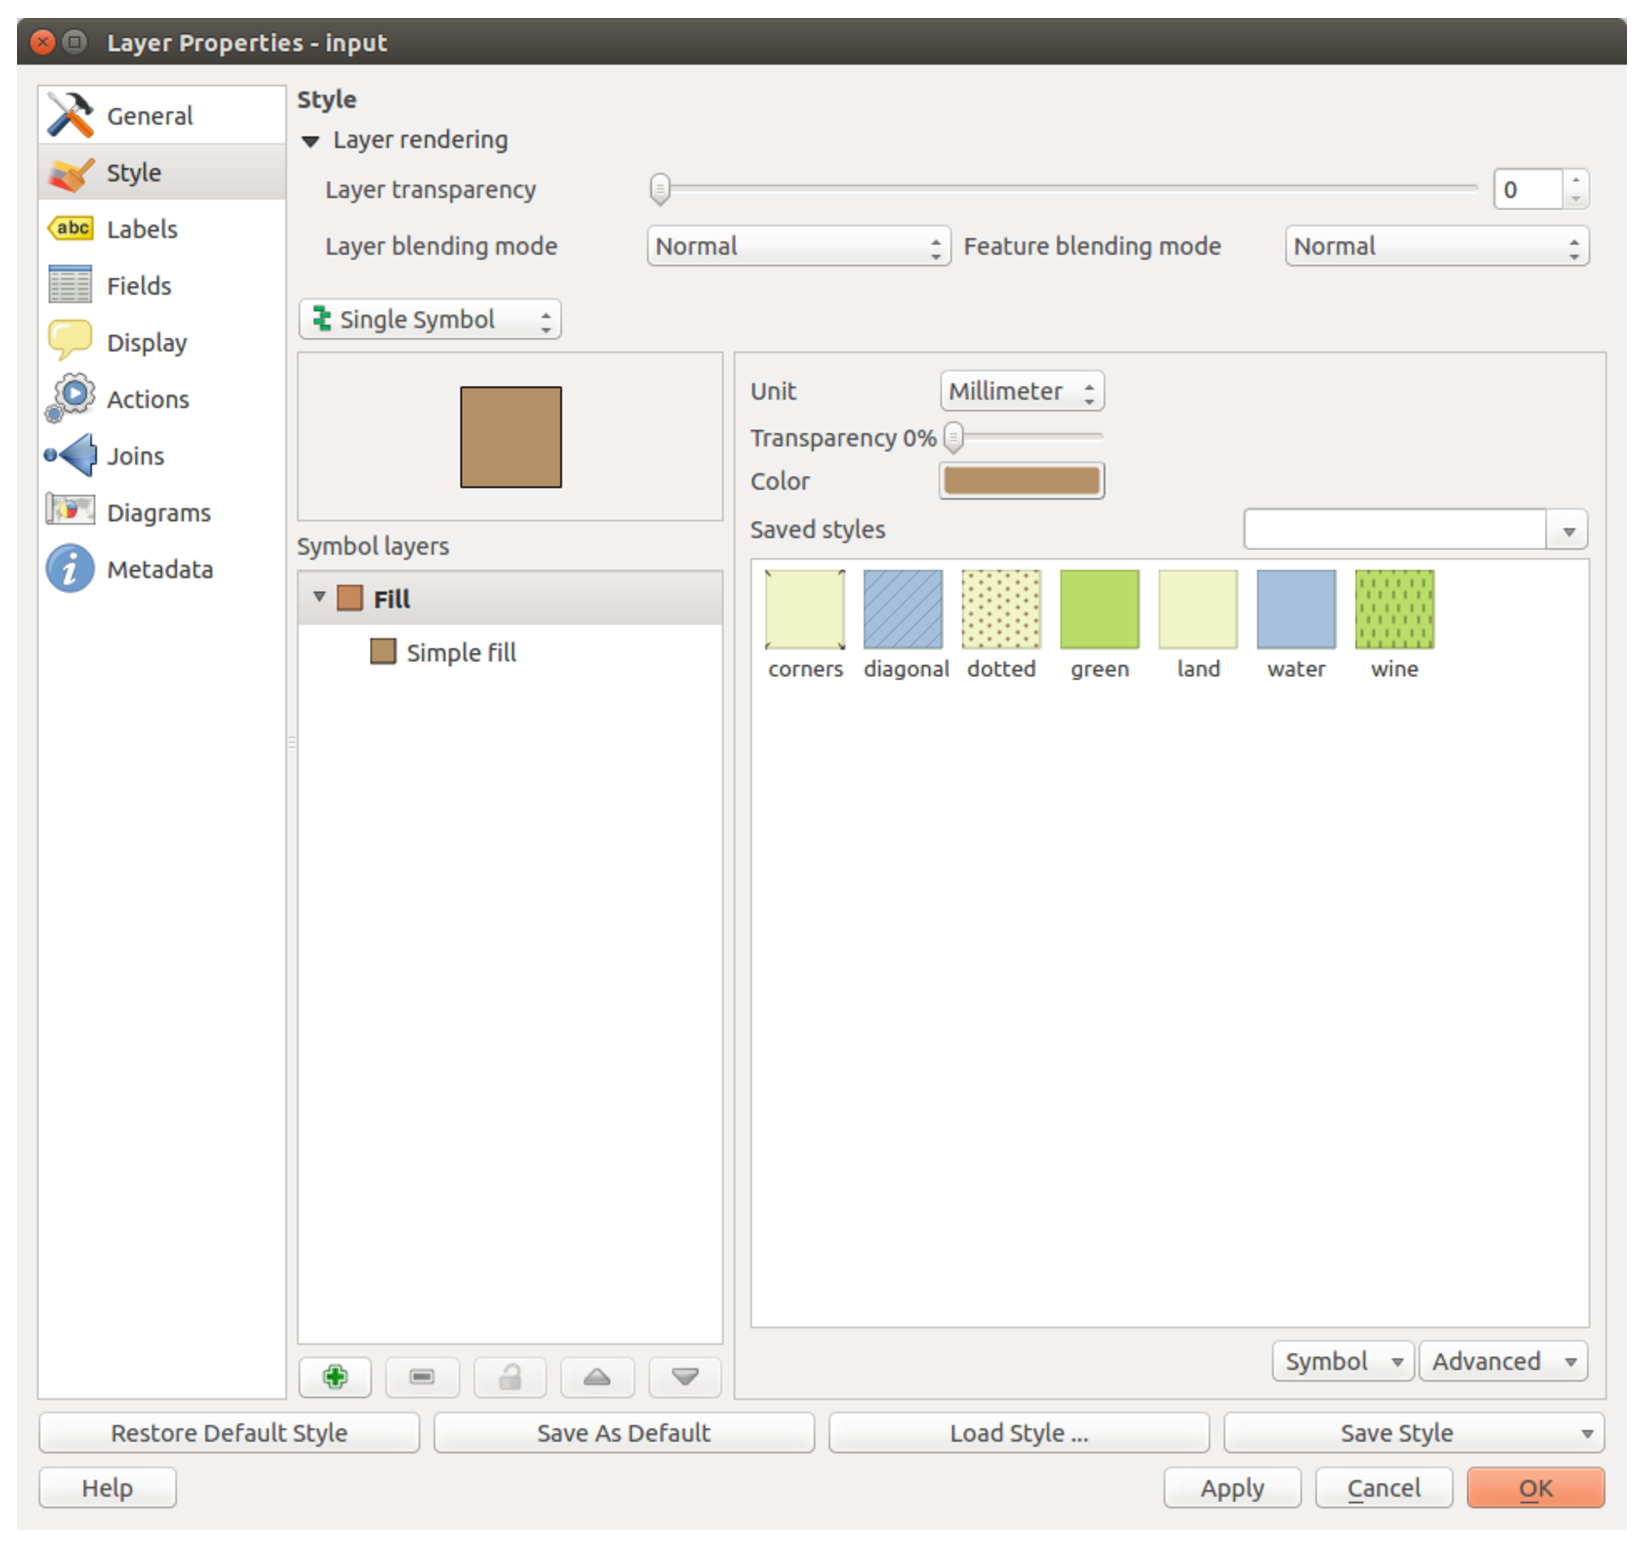
\includegraphics[scale=0.3]{propertybox} 
\caption{Properties box} 
\label{propertybox}
\end{figure}

Users can select ``graduated '' text and select the attribute to be displayed. The attribute here is the name of the column.

\begin{figure}[H]
\centering
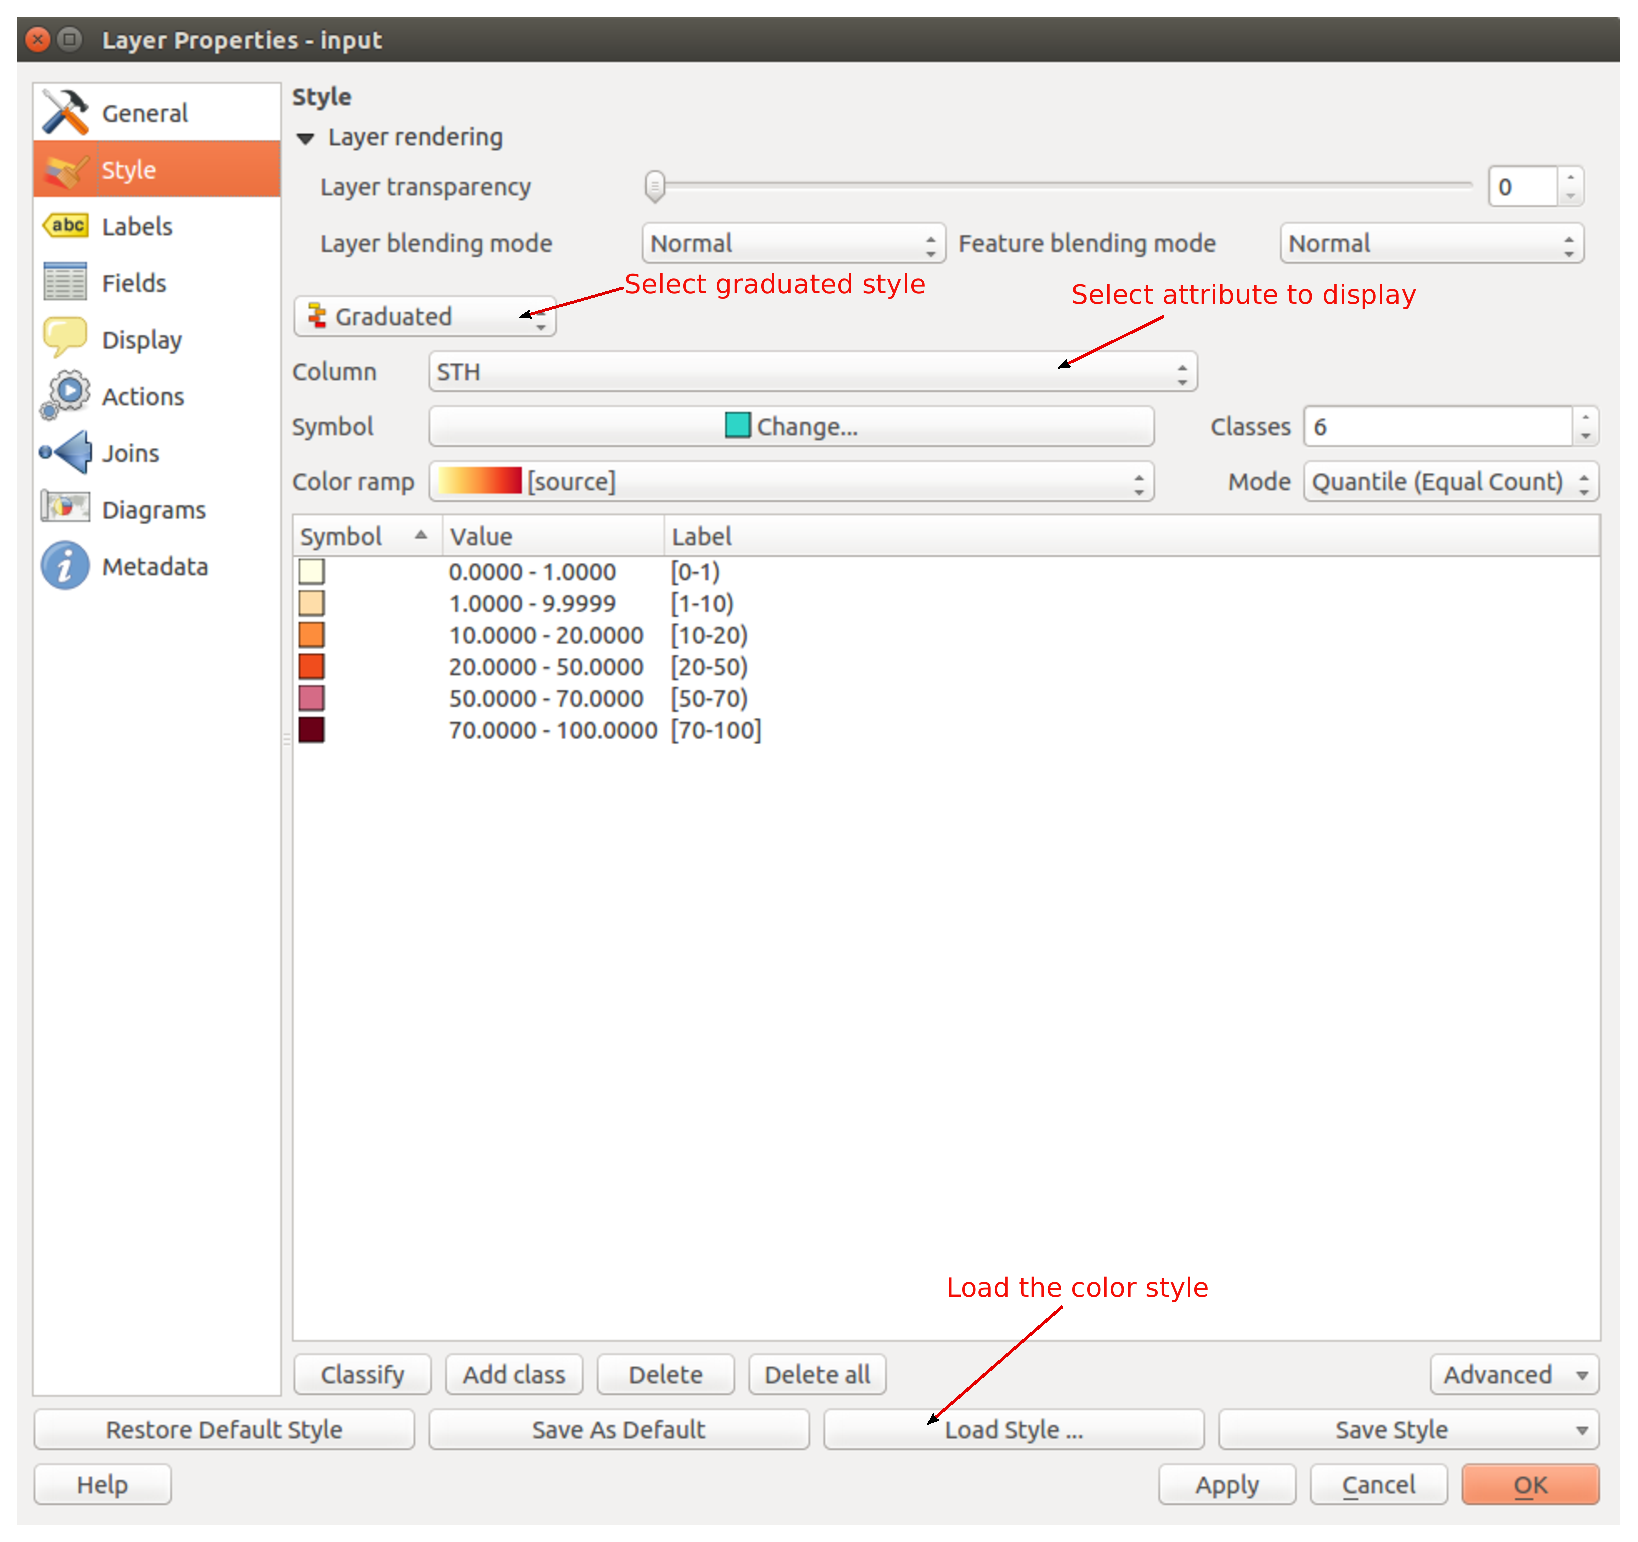
\includegraphics[scale=0.3]{propertyboxgraduate} 
\caption{Select graduate style and choose the attribute} 
\label{propertyboxgraduate}
\end{figure}

\subsubsection{Load/Define color properties}
Users can define a range of preferred colors for the map. For convenience of users, a default range of colors is predefined and it can be loaded (Figure \ref{propertyboxgraduate}).

The folder contains the default color style is shown in Figure \ref{colorstylefolder}
\subsubsection{Display results on QGIS}
Once the style is selected, the column name is defined, and the color style is loaded. Users can click the button ``Apply'' or ``OK'', the results will instantly display with different color on the map. 

Following figures show the prevalence at the origin (Figure \ref{outputsth0}) and after one year (Figure \ref{outputsth1})
\begin{figure}[H]
\centering
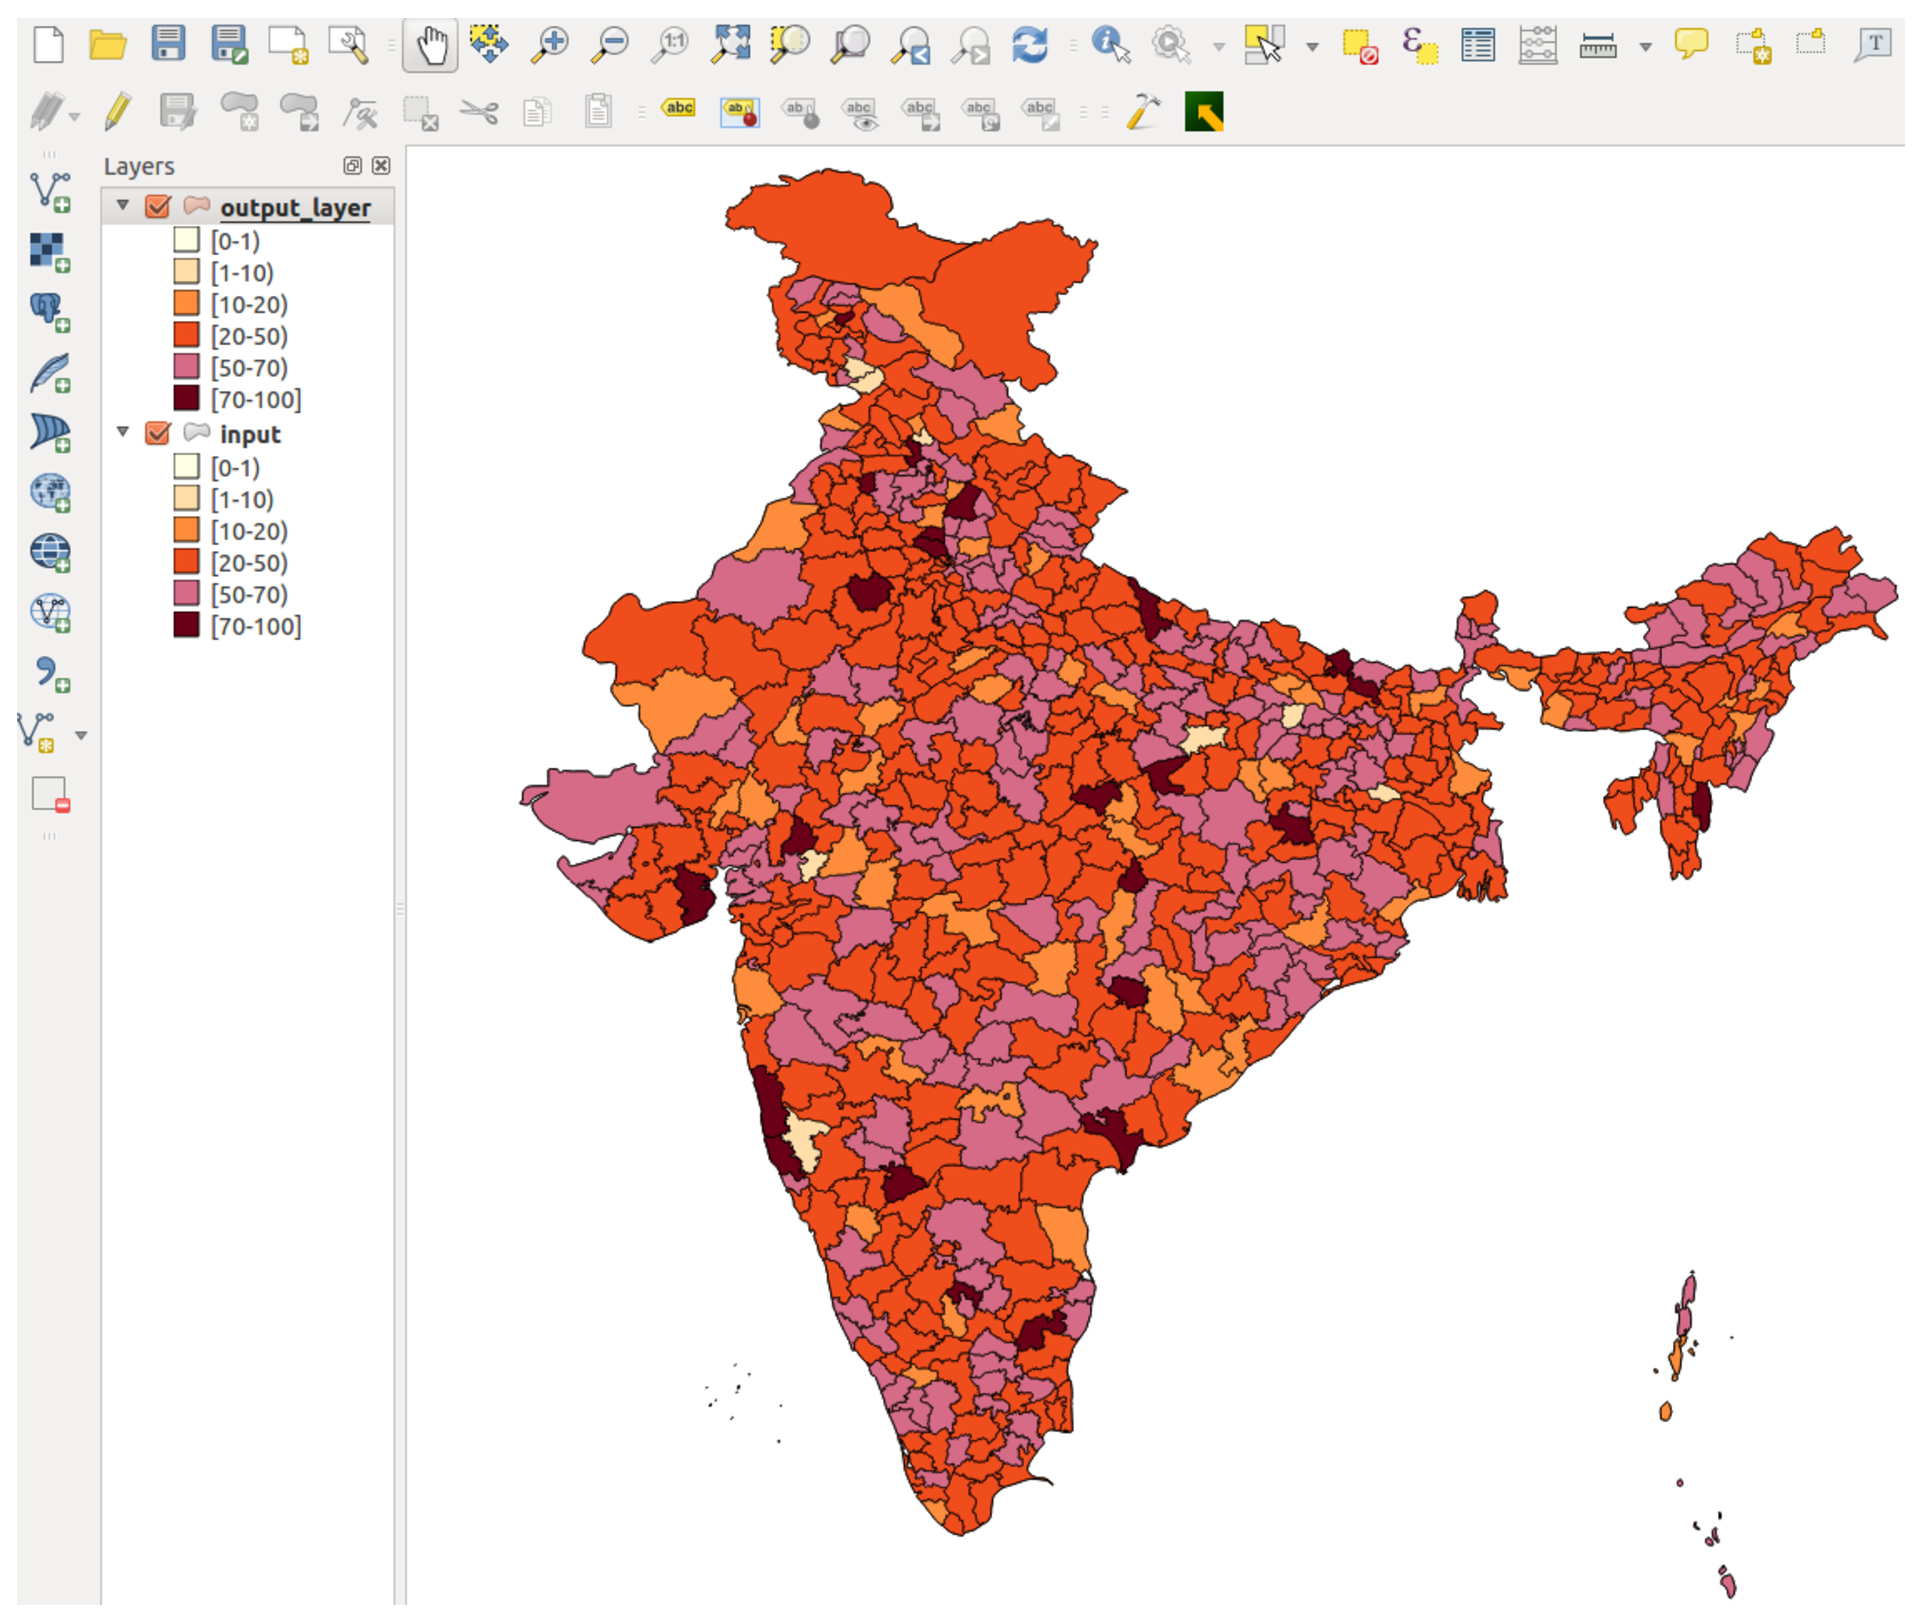
\includegraphics[scale=0.3]{outputsth0} 
\caption{Prevalence map at the initial time} 
\label{outputsth0}
\end{figure}

\begin{figure}[H]
\centering
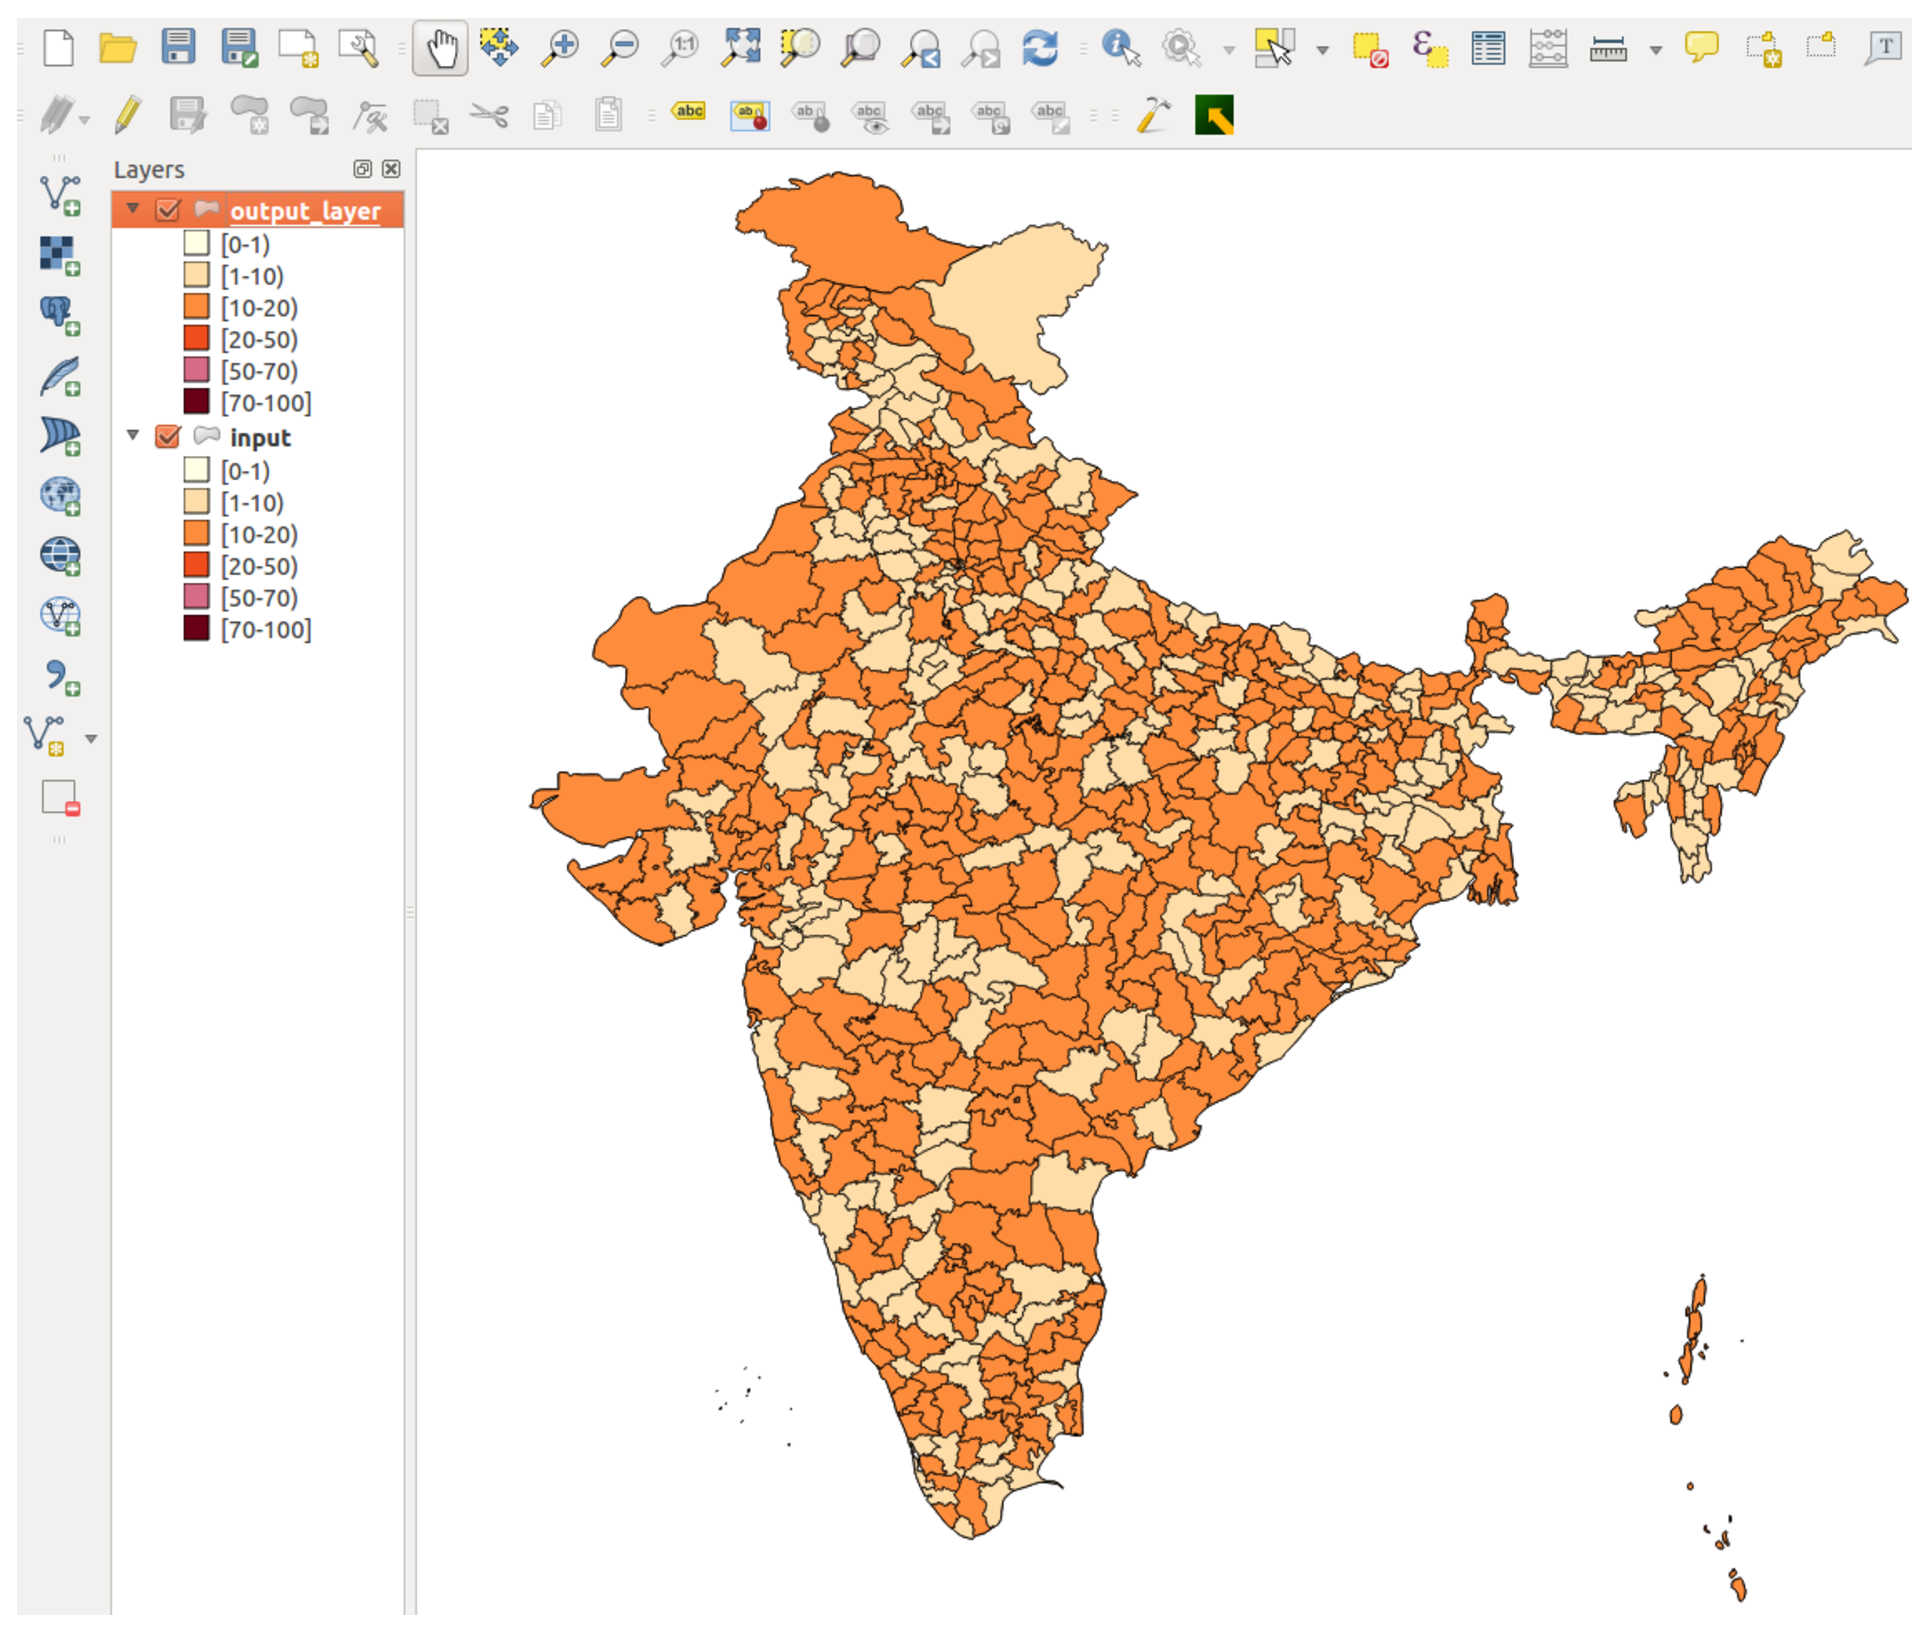
\includegraphics[scale=0.3]{outputsth1} 
\caption{Prevalence map at after one year} 
\label{outputsth1}
\end{figure}

As can be seen from the colored maps, there will be changes in total prevalence for entire India once the drug distribution programs (control programs) being implemented for each region.

\section*{3. Conclusion}
This STH-predictor was developed as a Python Plugin for QGIS. It works with shapefile with polygon structure. The modeling path of it was with Markov model \cite{Montresor2013}. There are two models built for the plugin. The default one is when there is only total prevalence of STH recorded. This case is phenomena in actual practice. The other model is used only when data on intensity level of Hookworms, \textit{Trichuris trichiura}, and \textit{Ascaris lumbricoides} is available. 

\section*{4. Acknowledgement}
This work was financially supported by the Ministry of Health of the Republic of Korea.

\begin{thebibliography}{9}
\bibitem{Montresor2013} 
Montresor, A.; Gabrielli, A. F.; Yajima, A.; Lethanh, N.; Biggs, B.-A.; Casey, G. J.; Tinh, T. T.; Engels, D. \& Savioli, L. \textit{``Markov model to forecast the change in prevalence of soil-transmitted helminths during a control programme: a case study in Vietnam''}. Transactions of The Royal Society of Tropical Medicine and Hygiene, 2013, 107, 313-318
\end{thebibliography}
\end{document}